\documentclass[aps,pra,reprint,superscriptaddress,floatfix]{revtex4-2}

\usepackage[T1]{fontenc}
\usepackage{amsmath,amssymb,amsthm}
\usepackage{graphicx}
\usepackage{bm}
\usepackage{xcolor}
\definecolor{linkblue}{HTML}{1F5FBF}
\definecolor{citemagenta}{HTML}{C0157D}
\usepackage[colorlinks=true,linkcolor=linkblue,citecolor=citemagenta,urlcolor=linkblue]{hyperref}
\usepackage{orcidlink}

\theoremstyle{plain}
\newtheorem{theorem}{Theorem}
\newtheorem{lemma}{Lemma}

\newcommand{\tr}{\operatorname{Tr}}
\newcommand{\ket}[1]{|#1\rangle}
\newcommand{\ketbra}[2]{|#1\rangle\!\langle #2|}
\newcommand{\nrm}[2]{\lvert #1\rvert_{#2}}
\newcommand{\Norm}[1]{\lVert #1\rVert}
\newcommand{\cD}{\mathcal D}
\newcommand{\cE}{\mathcal E}
\newcommand{\Nq}{\mathcal N_q}
\newcommand{\AD}{\mathcal{A\hspace{-0.6pt}D}}
\newcommand{\pnl}[1]{\textsf{\textbf{#1}}}

\hypersetup{
  pdftitle={The Memory Limits of Noisy Quantum Reservoirs},
  pdfauthor={Markus Baumann, Jonas Stein, Claudia Linnhoff-Popien},
  pdfsubject={Memory limits of quantum reservoirs with reinitialized inputs},
  pdfkeywords={quantum reservoir computing, memory, input reinitialization, depolarizing noise}
}

\begin{document}

\raggedbottom

\title{The Memory Limits of Noisy Quantum Reservoirs}

\author{Markus Baumann\,\orcidlink{0009-0007-3575-1006}}
\email[Contact author: ]{markus.baumann@campus.lmu.de}
\author{Jonas Stein\,\orcidlink{0000-0001-5727-9151}}
\author{Claudia Linnhoff-Popien\,\orcidlink{0000-0001-6284-9286}}
\affiliation{Quantum Applications and Research Laboratory (QAR-Lab), Department of Computer Science,
Ludwig-Maximilians-Universit\"at M\"unchen, Oettingenstra\ss e 67, 80538 M\"unchen, Germany}
\affiliation{Chair of Mobile and Distributed Systems, Department of Computer Science,
Ludwig-Maximilians-Universit\"at M\"unchen, Oettingenstra\ss e 67, 80538 M\"unchen, Germany}

\date{October 16, 2026}

\begin{abstract}
Quantum reservoir computing processes time series by injecting one input per time step into a fixed, noisy quantum system and training only a linear readout. A reservoir can solve a temporal task only if the inputs the task needs are still present in its state. What fundamentally limits this memory? Adding qubits seems the natural way to extend it. However, noise injects entropy into every qubit at every time step, and under depolarizing noise a reservoir can remove this entropy steadily only through the input qubits that are reinitialized at each time step. Here we show that this number, not the size of the reservoir, sets the memory. With $k$ reinitialized input qubits per time step, the largest attainable memory depth at fixed accuracy is $\exp[\Theta(k)]$ time steps once the initial state has been washed out, independent of the total number of qubits. The upper bound holds for every reservoir unitary and input encoding, and an explicit construction shows that the exponential scaling is attainable. Retaining an input for $T$ time steps therefore requires $\Theta(\log T)$ reinitialized input qubits per time step. Unital noise leaves this limit unchanged, whereas non-unital noise acts as an additional entropy sink. These results identify reinitialized input qubits, not reservoir size, as the fundamental resource for memory in quantum reservoir computing, and make memory a quantity that can be budgeted in the design of quantum reservoirs.
\end{abstract}

\maketitle

%======================================================================
\section{Introduction}
%======================================================================

Reservoir computing (RC) processes sequential data with the transient dynamics of a fixed nonlinear system, the \emph{reservoir}, and trains only a linear readout~\cite{Jaeger2001,Maass2002,JaegerHaas2004,Lukosevicius2009}. Because training reduces to linear regression, the reservoir can be any physical system with suitable dynamics~\cite{Tanaka2019}. Quantum reservoir computing (QRC) uses quantum systems for this purpose, motivated by the large state space of interacting qubits~\cite{Fujii2017,Nakajima2019,Mujal2021}. Quantum reservoirs and the closely related quantum extreme learning machines have been realized on superconducting processors with up to 124 qubits~\cite{Chen2020,Suzuki2022,Yasuda2023,Hu2024,Monzani2024,Dao2026}.

\begin{figure*}[t]
\centering
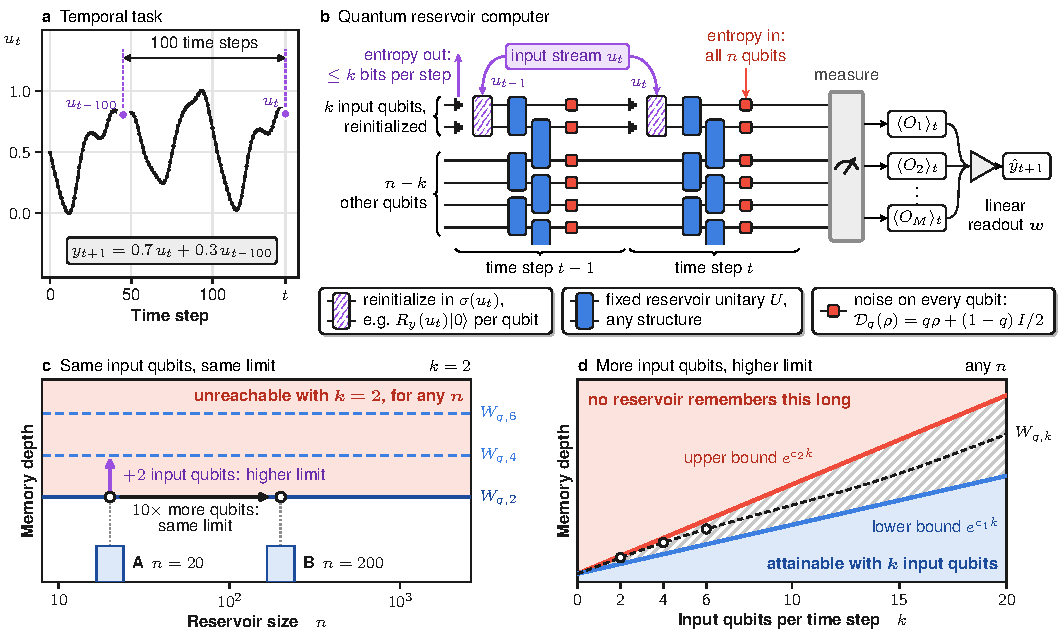
\includegraphics{fig1.pdf}
\caption{\textbf{Quantum reservoir computing with input injection by reinitialization, and its memory limit.}
\pnl{a}~A temporal task. Forecasting $y_{t+1}=0.7\,u_t+0.3\,u_{t-100}$ requires the reservoir to retain every input for 100 time steps (input stream: a Mackey--Glass series rescaled to $[0,1]$).
\pnl{b}~A noisy quantum reservoir. At every time step, the $k$ qubits of the input register are discarded and reinitialized in a state $\sigma(u_t)$ that encodes the input (hatched purple blocks), a fixed reservoir unitary $U$ acts on all $n$ qubits (blue blocks; the brickwork is only an example), and every qubit undergoes depolarizing noise (red). A trained linear readout combines expectation values $\langle O_i\rangle_t$ into the prediction $\hat y_{t+1}$. Note the imbalance: noise injects entropy into all $n$ qubits at every time step, whereas only the $k$ discarded input qubits carry entropy out.
\pnl{c}~Two reservoirs with the same number of input qubits, $k=2$, and the same noise, but with $n=20$ (A) and $n=200$ (B) qubits. Neither can exceed the largest memory depth $W_{q,2}$ of any reservoir with two input qubits: ten times more qubits do not move this limit, whereas two more input qubits raise it. The bars indicate the memory depths of A and B; they are drawn equal because, in the simulations of Sec.~\ref{sec:numerics}, the memory depth does not grow with $n$.
\pnl{d}~The content of Theorem~\ref{thm:main}: the limit $W_{q,k}$ lies between two exponentials in $k$, for every $n$. No reservoir remembers longer than the upper bound, and the reservoir of Sec.~\ref{sec:lower} remembers at least as long as the lower bound; the hatched gap reflects the constants of the two bounds. Panels \pnl{c} and \pnl{d} are schematic. Colors have the same meaning in all figures: purple marks the input, blue the reservoir dynamics and attainable memory, red the noise and the limit, and grey neutral elements such as standard reservoirs and reference curves.}
\label{fig:overview}
\end{figure*}

For temporal tasks, memory is the central resource. Consider forecasting a time series whose next value depends on an input from 100 time steps ago [Fig.~\ref{fig:overview}\,\pnl{a}],
\begin{equation}
y_{t+1}=0.7\,u_t+0.3\,u_{t-100}.
\label{eq:task}
\end{equation}
A reservoir can solve this task only if $u_{t-100}$ still influences its state at time $t$. Once the reservoir has forgotten this input, no readout can recover it, however well it is trained. The memory of a reservoir is commonly characterized by the echo-state and fading-memory properties, which guarantee that old inputs eventually lose their influence~\cite{Jaeger2001,Boyd1985,MartinezPena2023}, and it is quantified by memory capacities~\cite{Jaeger2002}.

On current hardware, noise makes memory a bottleneck, because every qubit is degraded at every time step. An experimenter who wants a longer memory has several options: add qubits, change the couplings, inject the input differently, reduce the noise, or reinitialize more qubits at each time step. Each of these options may help in a given device, but it is unclear which of them can extend the memory without limit. This raises a basic question about resources: \emph{Can a quantum reservoir store past inputs for arbitrarily long by adding qubits, or is its memory limited by the number of qubits that are freshly prepared at each time step?}

The answer is not obvious, because the memory of a reservoir is not simply the coherence time of its qubits. A large reservoir can protect information: it can store an input redundantly and keep correcting the errors that noise introduces. Correcting errors, however, does not destroy the entropy that noise produces; it only moves this entropy elsewhere. In a reservoir with fixed dynamics and no feedback, the natural place for this entropy is the set of qubits that are discarded and reinitialized when a new input is injected [Fig.~\ref{fig:overview}\,\pnl{b}]. Input injection by reinitialization is the scheme of the original QRC proposal~\cite{Fujii2017}, and it also underlies protocols that measure and reset part of the reservoir at every time step~\cite{Yasuda2023,Hu2024}. A reservoir therefore resembles a leaking boat: a larger boat takes longer to sink, but it stays afloat only if water is bailed out as fast as it comes in, and the reinitialized input qubits are the bucket.

Several elements of an answer are known. Criteria for the echo-state and fading-memory properties guarantee that old inputs eventually lose their influence~\cite{MartinezPena2023,MorguiSancho2026}, and Markovian reservoirs forget at an exponential rate~\cite{Sannia2026}. These results do not tell, however, whether forgetting takes ten time steps or a million, nor how this time depends on the available resources. Dissipation and non-unital noise have been identified as resources for QRC in theory and experiment~\cite{Chen2020,Kubota2023,Sannia2024,Monzani2024}, including collective relaxation as a scalable source of fading memory~\cite{Freiheit2026}, and mid-circuit measurements with resets allow a reservoir to process data streams far longer than the coherence time of its qubits~\cite{Yasuda2023,Hu2024}. Running indefinitely is not the same as remembering for long, though: a reservoir can operate forever and still use only its last ten inputs. In noisy quantum computation, it is well established that noise limits the effective depth of circuits and that fresh qubits are essential, because without them depolarizing noise permits only logarithmically long computations~\cite{Aharonov1996,BenOr2013,StilckFranca2021,Mele2026}. What has been missing is a quantitative relation between the resources of a quantum reservoir and the longest memory it can achieve, valid for every reservoir dynamics.

In this work, we establish this relation. We consider a reservoir of $n$ qubits in which $k$ input qubits are reinitialized at every time step and every qubit undergoes depolarizing noise of strength $q$. We define the \emph{memory depth} $W(\varepsilon)$ as the number of past time steps whose inputs still influence the reservoir state beyond an accuracy $\varepsilon$, and we denote by $W_{q,k}(\varepsilon)$ the largest memory depth that any such reservoir can reach, whatever its size, reservoir unitary, and input encoding. Our main result is
\begin{equation}
W_{q,k}(\varepsilon)=\exp\!\big[\Theta_q(k)\big].
\label{eq:main}
\end{equation}
For fixed noise and accuracy, and once the initial state has been washed out, there are constants $c_1,c_2>0$ that depend only on $q$ such that $e^{c_1k}\le W_{q,k}(\varepsilon)\le e^{c_2k}$ for all sufficiently large $k$ [Fig.~\ref{fig:overview}\,\pnl{d}]. The lower bound states that a reservoir can be built that remembers for a time exponential in $k$. The upper bound states that no reservoir can remember longer than exponentially in $k$. The total number of qubits $n$ does not appear.

Equation~\eqref{eq:main} has a simple consequence [Fig.~\ref{fig:overview}\,\pnl{c}]. A reservoir A with 20 qubits and a reservoir B with 200 qubits, both with two input qubits reinitialized per time step and the same noise, are subject to the same memory limit; the tenfold larger reservoir B cannot exceed the limit that also binds A, whereas two more input qubits raise it. Turned around, retaining an input for $T$ time steps requires, and can be achieved with, $k=\Theta_q(\log T)$ reinitialized input qubits per time step. Exponentially more memory needs only linearly more input qubits, and not even the best conceivable reservoir can do with fewer.

The upper bound holds for every reservoir unitary, local or nonlocal, entangling or not, and for every input encoding and readout. It rests on a single distance between reservoir states that every noisy time step contracts by the same factor, whatever the dynamics. The lower bound is a reservoir that stores its input in a repetition code and refreshes it by majority vote; it uses classical reversible logic and at most $2k$ qubits, and it serves as a proof device rather than as a proposal for practical QRC. Beyond depolarizing noise, the result becomes an entropy budget. Unital noise and measurements of the reservoir qubits without feedback cannot extend the limit, whereas non-unital noise such as energy relaxation acts as an additional entropy sink and can make the memory grow with the reservoir size. Finally, simulations of standard reservoirs show how far they operate below the limit: a transverse-field Ising reservoir with $n=8$ qubits remembers about 12 time steps at $q=0.9$, for every size we simulated, whereas the reservoir that reaches the limit remembers 316 time steps with the same number of qubits.

The paper is organized as follows. Section~\ref{sec:model} introduces the model and states the main theorem. Section~\ref{sec:upper} explains why no reservoir can remember longer, and Sec.~\ref{sec:lower} presents a reservoir that reaches the limit. Section~\ref{sec:discussion} compares standard reservoirs with the limit and discusses the implications for reservoir design, the role of the noise assumptions, and what the result does not imply. Section~\ref{sec:conclusions} concludes. The Appendices contain the proofs, exact results for the constructions, and the details of the simulations.

%======================================================================
\section{Model and main theorem}
\label{sec:model}
%======================================================================

\subsection{Quantum reservoir with input injection by reinitialization}

We consider a reservoir of $n$ qubits driven by a sequence of classical inputs $u_t$, one per time step $t$ [Fig.~\ref{fig:overview}\,\pnl{b}]. The qubits are divided into an \emph{input register} of $k$ qubits and the remaining $n-k$ qubits. Each time step consists of three operations. In the \emph{input injection}, the input register is reinitialized: its previous state is discarded and replaced by an \emph{input state} $\sigma(u_t)$ that encodes $u_t$. In the \emph{reservoir dynamics}, a fixed reservoir unitary $U$ acts on all $n$ qubits. Finally, every qubit undergoes depolarizing \emph{noise},
\begin{equation}
\cD_q(\rho)=q\,\rho+(1-q)\tr(\rho)\,\frac I2,\qquad0<q<1,
\label{eq:depol}
\end{equation}
which leaves the qubit untouched with probability $q$ and replaces its state by the completely mixed state otherwise. The reservoir state therefore evolves as
\begin{equation}
\rho_t=\cD_q^{\otimes n}\Bigl(U\bigl[\sigma(u_t)\otimes\tr_{\mathrm{in}}\rho_{t-1}\bigr]U^\dagger\Bigr),
\label{eq:model}
\end{equation}
where $\tr_{\mathrm{in}}$ denotes the partial trace over the input register. The reservoir output consists of expectation values $r_{t,i}=\tr(O_i\rho_t)$ of a set of observables with $\Norm{O_i}\le1$, and a trained linear readout combines them into a prediction $\hat y_{t+1}=\bm w\cdot\bm r_t$.

This model contains the input injection of the original QRC proposal, in which one qubit is reinitialized per time step~\cite{Fujii2017}, and measurement-based schemes in which $k$ qubits are measured and reset at every time step, provided that the measurement outcomes are not fed back into the reservoir~\cite{Yasuda2023,Hu2024}. The input state $\sigma(u)$ is arbitrary; it may encode the input in only some of the $k$ qubits and prepare the others in a fixed state. We impose no restriction on the reservoir unitary: $U$ may be local or nonlocal, shallow or deep, entangling or not.

\paragraph*{Where the input qubits enter.}
The $k$ input qubits enter our analysis through a single property of the injection step. Because $\sigma(u)\le I$, the map $\cE_u(X)=U[\sigma(u)\otimes\tr_{\mathrm{in}}X]U^\dagger$ that combines input injection and reservoir dynamics obeys
\begin{equation}
\cE_u(I)\le2^k\,I .
\label{eq:budget}
\end{equation}
In words, one time step can lower the entropy of a completely mixed reservoir by at most $k$ bits (more precisely, its min-entropy). We say that the injection step has a \emph{budget} of $k$ bits (Appendix~\ref{app:norms}). Equation~\eqref{eq:budget} is the formal counterpart of the bucket in the leaking-boat picture. It is the only property of the injection step that our upper bound uses, so the bound also covers input-dependent reservoir unitaries.

\subsection{Echo states and memory depth}

A reservoir has the \emph{echo-state property} if it forgets its initial state, so that an input sequence $h=(\dots,u_{-1},u_0)$ extending into the infinite past determines a unique reservoir state $\rho(h)$, the \emph{echo state}~\cite{Jaeger2001,MartinezPena2023}. Every reservoir of the form~\eqref{eq:model} has this property (Sec.~\ref{sec:upper}).

We measure memory by how far back the echo state still depends on the inputs. The \emph{memory depth} $W(\varepsilon)$ is the smallest number $L$ of time steps such that any two input sequences that agree on their last $L$ inputs lead to echo states within trace distance $\varepsilon$,
\begin{equation}
\tfrac12\Norm{\rho(h)-\rho(h')}_1\le\varepsilon .
\label{eq:depth}
\end{equation}
Inputs older than $W(\varepsilon)$ time steps change every output $r_{t,i}$ by at most $2\varepsilon$, so no readout can extract more than that from them; inputs within the memory depth can still matter. The memory capacity~\cite{Jaeger2002} measures how well one particular linear readout reconstructs past inputs. The memory depth, in contrast, is a property of the reservoir state and limits all readouts at once. We denote by $W_{q,k}(\varepsilon)$ the largest memory depth of any reservoir with $k$ input qubits and noise strength $q$, maximized over the number of qubits, the reservoir unitary, and the input encoding. Table~\ref{tab:notation} summarizes the notation.

\begin{table}[b]
\caption{Notation used throughout this work.}
\label{tab:notation}
\begin{ruledtabular}
\begin{tabular}{p{1.75cm}p{5.85cm}}
{\centering Symbol\par} & {\raggedright Meaning\par} \\ \hline
{\centering $n$\par} & {\raggedright total number of qubits of the reservoir\par} \\
{\centering $k$\par} & {\raggedright number of input qubits reinitialized at every time step\par} \\
{\centering $q$\par} & {\raggedright noise strength: depolarizing noise keeps the state of each qubit with probability $q$ per time step\par} \\
{\centering $\varepsilon$\par} & {\raggedright accuracy: inputs that change the reservoir state by less than $\varepsilon$ in trace distance count as forgotten\par} \\
{\centering $W(\varepsilon)$\par} & {\raggedright memory depth: number of past time steps whose inputs still change the reservoir state by more than $\varepsilon$\par} \\
{\centering $W_{q,k}(\varepsilon)$\par} & {\raggedright largest memory depth of any reservoir with $k$ input qubits and noise strength $q$, for any $n$, reservoir unitary, and input encoding\par} \\
{\centering $O_q,\Omega_q,\Theta_q$\par} & {\raggedright bounded from above, from below, or from both sides by constant multiples of the argument, with constants that depend only on $q$; for example, $\Theta_q(k)$\par} \\
\end{tabular}
\end{ruledtabular}
\end{table}

\subsection{Main theorem}

\begin{theorem}[Memory limit]\label{thm:main}
Fix the noise strength $0<q<1$ and an accuracy $0<\varepsilon<q$. Every reservoir with $k$ input qubits reinitialized per time step has memory depth
\begin{equation}
W(\varepsilon)\le\Bigl\lceil A_q\,2^{\beta_qk}\ln\frac1\varepsilon\Bigr\rceil,
\label{eq:upper}
\end{equation}
whatever its number of qubits, reservoir unitary, and input encoding. Conversely, for every $k\ge k_q$ there is a reservoir with at most $2k$ qubits whose memory depth satisfies
\begin{equation}
W(\varepsilon)\ge\frac14\,e^{\alpha_q(k-3)}\ln\frac q\varepsilon .
\label{eq:lowerthm}
\end{equation}
The constants depend only on $q$:
\begin{gather}
\alpha_q=-\tfrac12\ln(1-q^2),\qquad\beta_q=\frac{q(1+q^2)}{(1-q)(1-q^2)},\nonumber\\
\log_2A_q=\frac1{1-q}\Bigl[1+\frac{2q(3-q^2)}{1-q^2}\Bigr],\qquad k_q=3+\Bigl\lceil\frac{\ln4}{\alpha_q}\Bigr\rceil.
\label{eq:thmconstants}
\end{gather}
\end{theorem}

\paragraph*{Where the constants come from.}
None of the constants is a fit parameter; each has a simple origin, derived in the Appendices and collected in Table~\ref{tab:constglossary}. The exponent $\alpha_q$ of the lower bound is the rate at which a majority vote over $r$ noisy copies becomes reliable: the vote fails with probability at most $e^{-\alpha_qr}$ per time step (Sec.~\ref{sec:lower}). The exponent $\beta_q$ of the upper bound tells how much the time over which a reservoir forgets can grow, in bits, per input qubit, and $A_q$ collects the factors that do not depend on $k$ (Appendix~\ref{app:constants}). The threshold $k_q$ is a sufficient number of input qubits for the majority vote to be reliable enough for the lower bound (Appendix~\ref{app:lowerbound}), and the condition $\varepsilon<q$ reflects the last round of noise on the readout qubit. At $q=0.9$, $\alpha_q=0.83$, $\beta_q=85.7$, $\log_2A_q=217.5$, and $k_q=5$.

\paragraph*{What the theorem says.}
Both bounds grow exponentially with $k$, and neither depends on $n$; this is Eq.~\eqref{eq:main}, illustrated in Figs.~\ref{fig:overview}\,\pnl{c} and \ref{fig:overview}\,\pnl{d}. Every additional input qubit raises the upper bound by the factor $2^{\beta_q}$, and the reservoir of Sec.~\ref{sec:lower} gains a constant factor per input qubit as well. Because the two exponents differ, the theorem fixes how the memory scales with $k$, not the exact rate. Since the lower bound requires only $n\le2k$ qubits, qubits beyond $2k$ can improve the memory depth at most by changing the constant in the exponent.

Two remarks delimit the statement. First, the theorem concerns echo states, that is, inputs injected after the initial state has been washed out. The initial state is a separate resource: it can hold $n$ redundant copies of a bit, which take $\Theta_q(\log n)$ time steps to wash out (Appendix~\ref{app:washout}). A larger reservoir thus needs a longer washout, but it cannot remember new inputs for longer. Second, the constants are far from tight (Appendix~\ref{app:upper}). At $q=0.9$, the upper bound is $A_q2^{\beta_qk}\ln(1/\varepsilon)\approx2^{217+86k}\ln(1/\varepsilon)$, so it gains a factor of $2^{86}$ per input qubit, whereas the reservoir of Sec.~\ref{sec:lower} gains a factor of about five for every two additional input qubits. Theorem~\ref{thm:main} is therefore a statement about scaling and about the limiting resource, not a formula for the memory of a specific device.

%======================================================================
\section{Why no reservoir can remember longer}
\label{sec:upper}
%======================================================================

\begin{figure*}[t]
\centering
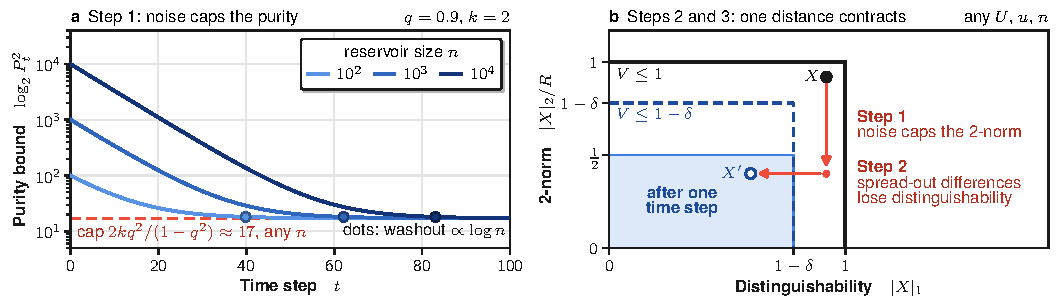
\includegraphics{fig2.pdf}
\caption{\textbf{Why every reservoir forgets.}
\pnl{a}~Step~1, computed. Upper bound~\eqref{eq:purity} on the purity, in pure qubits' worth, of reservoirs with $k=2$ input qubits at $q=0.9$ that start in a pure state of $n$ qubits. Whatever the reservoir size, the bound falls to the same cap $2kq^2/(1-q^2)\approx17$ (dashed). Dots mark the washout, after which the bound stays within one bit of the cap; it grows only as $\log n$.
\pnl{b}~Steps~2 and 3, schematic. A point represents the difference $X$ between two reservoir states, placed by its distinguishability and its 2-norm. One time step maps every point of the box $V\le1$ into the shaded region, as shown for one difference $X$ and its image $X'$: noise caps the 2-norm (Step~1), and spread-out differences lose a fixed fraction of their distinguishability (Step~2). The shaded region lies inside the dashed box $V\le1-\delta$ for every reservoir unitary, input, and reservoir size, so every time step shrinks $V$ by the factor $1-\delta$ (Step~3). The size of $\delta$ is exaggerated for visibility.}
\label{fig:contraction}
\end{figure*}

The intuition behind the upper bound is simple. Noise destroys information at every time step. A reservoir can repair the damage only by dumping entropy into its input register, and $k$ reinitialized qubits can absorb only a bounded amount of entropy per time step. Turning this intuition into a proof is harder than it seems, because a general reservoir can hide information much better than a list of copies. It can spread an input over many qubits, entangle it, and use its input qubits for repair in ways nobody has thought of. A proof must defeat all such strategies at once, without knowing the reservoir unitary.

Our proof follows two reservoir states $\rho$ and $\rho'$ that arose from different input histories. It tracks two properties of their difference $X=d(\rho-\rho')$, where $d=2^n$. The first is the \emph{distinguishability} $\nrm X1=\Norm{\rho-\rho'}_1$, which bounds how well any measurement can tell the two states apart. The second is the 2-norm $\nrm X2$, which is small when both states are close to the completely mixed state. Here $\nrm Xp=(d^{-1}\tr|X|^p)^{1/p}$ denotes the Schatten norm normalized so that $\nrm Ip=1$. For a single state, $P=\nrm{d\rho}2=(d\tr\rho^2)^{1/2}$ measures the purity: a state with $m$ pure qubits and $n-m$ completely mixed ones has $P^2=2^m$, so $\log_2P^2$ counts pure qubits' worth of purity (Appendix~\ref{app:norms}). Two established inequalities about depolarizing noise drive the argument~\cite{King2014,Cubitt2015}.

\paragraph*{Step 1: Noise caps the purity.}
Depolarizing noise is hypercontractive~\cite{King2014}: it turns operators with a bounded $(1+q^2)$-norm into operators with a bounded 2-norm, because it damps the many-qubit correlations that make an operator concentrated. By Eq.~\eqref{eq:budget}, the injection step can raise the 2-norm by at most a factor $2^{k/2}$. Together, the purity obeys
\begin{equation}
\ln P_t\le\theta\ln P_{t-1}+\frac{\theta k}2\ln2,\qquad\theta=\frac{2q^2}{1+q^2}<1 .
\label{eq:purity}
\end{equation}
The exponent $\theta$ arises because the $(1+q^2)$-norm lies between the 1-norm and the 2-norm; interpolating between them gives the power $\theta$ (Appendix~\ref{app:cap}). The log-purity thus has a fading memory of its own: every time step multiplies it by $\theta<1$, and the input qubits add at most a constant. Its fixed point is $P_*=2^{kq^2/(1-q^2)}$. After $O_q(\log n)$ time steps, the purity stays below $\sqrt2P_*$, and echo states obey $P\le P_*$ [Fig.~\ref{fig:contraction}\,\pnl{a}]. In words, the echo state of any reservoir, whatever its size, holds at most $2kq^2/(1-q^2)$ pure qubits' worth of purity, about $8.5$ per input qubit at $q=0.9$. The time it takes to reach this bound is the washout of the initial state.

\paragraph*{Step 2: Bounded purity forces forgetting.}
A bounded purity alone does not imply forgetting. The two states $\ketbra bb\otimes I/2^{n-1}$, $b=0,1$, have almost minimal purity, yet they are perfectly distinguishable. What a bounded purity does imply is that such distinguishability cannot survive the next layer of noise. Reverse hypercontractivity~\cite{Cubitt2015} states that depolarizing noise forces positive operators to overlap. Applied to the positive and negative parts of $X$, it shows that every measurement confuses $\rho$ with $\rho'$ with a probability bounded from below whenever $X$ is spread out, that is, whenever $\nrm X2$ is not much larger than $\nrm X1$. One layer of noise then destroys a fixed fraction of the distinguishability (Lemma~\ref{lem:forget} in Appendix~\ref{app:upper}).

\paragraph*{Step 3: One distance contracts.}
Neither step suffices on its own: Step~1 controls the purity but not the distinguishability, and Step~2 needs the control that Step~1 provides. Combined, they yield a single distance between reservoir states, $V(X)=\max\{\nrm X1,\nrm X2/R\}$, that every time step contracts [Fig.~\ref{fig:contraction}\,\pnl{b}]. The weight $R$ puts the 2-norm on the scale of the 1-norm; it depends only on $q$ and $k$ and is chosen such that one noisy time step at least halves the 2-norm part of $V$ (Appendix~\ref{app:contract}). The contraction reads
\begin{equation}
V\bigl(\cD_q^{\otimes n}\cE_uX\bigr)\le(1-\delta)\,V(X),\qquad\delta^{-1}=A_q\,2^{\beta_qk}.
\label{eq:contraction}
\end{equation}
Here $\delta$ is the fraction of $V$ that every time step removes, with the constants $A_q$ and $\beta_q$ of Eq.~\eqref{eq:thmconstants}. It depends only on $q$ and $k$, not on $n$, on the inputs, or on the reservoir unitary (Appendix~\ref{app:upper}).

The memory limit follows at once. Contraction implies that every infinite input sequence drives the reservoir into a unique echo state. Two input sequences that agree on their last $L$ inputs lead to echo states with
\begin{equation}
\tfrac12\Norm{\rho(h)-\rho(h')}_1\le e^{-\delta L},
\label{eq:forget}
\end{equation}
so the memory depth is at most $\lceil\delta^{-1}\ln(1/\varepsilon)\rceil$, which is the upper bound~\eqref{eq:upper}. Whatever a reservoir does with its qubits, every time step erases a fixed fraction of its past, and only the number of reinitialized input qubits determines how small that fraction can be made.

\paragraph*{What the proof uses, and what it does not.}
The argument uses three ingredients: one layer of independent depolarizing noise per time step, the budget inequality~\eqref{eq:budget}, and the fact that unitary dynamics preserves both norms. It never uses locality, the structure of $U$, or the encoding of the input. The same argument also covers the case $k=0$, a reservoir whose input enters only through an input-dependent unitary. Such a reservoir has no entropy sink at all: the completely mixed state is a common fixed point of all its time steps, so by contraction its echo state is the completely mixed state for every input sequence. Under depolarizing noise, a reservoir with purely unitary input encoding therefore retains nothing once the initial state has been washed out. This is consistent with the observation that contractive reservoirs with input-independent fixed points carry no information about their inputs~\cite{MartinezPena2023}, and with the role of dissipation as a resource for QRC~\cite{Chen2020,Sannia2024,Monzani2024}.

%======================================================================
\section{A reservoir that reaches the limit}
\label{sec:lower}
%======================================================================

\begin{figure*}[t]
\centering
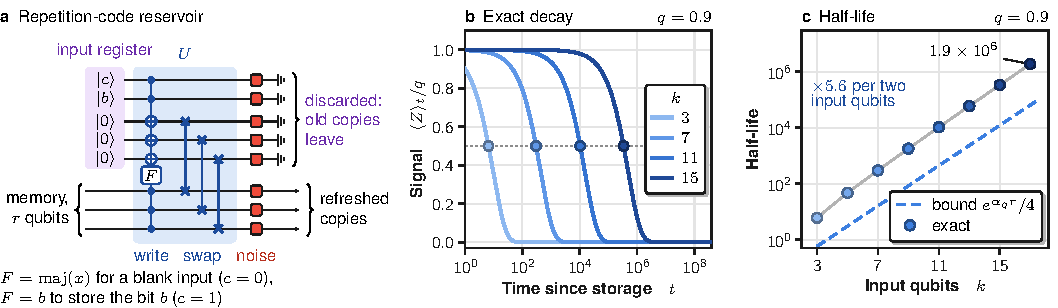
\includegraphics{fig3.pdf}
\caption{\textbf{A reservoir that reaches the memory limit.}
\pnl{a}~One time step of the repetition-code reservoir for $r=3$ memory qubits ($k=5$ input qubits). The input register holds two qubits $\ket{c,b}$ that encode the input and $r$ ancillas reinitialized in $\ket0$. The write gate computes $F=b$ (store, $c=1$) or $F=\mathrm{maj}(x)$ (blank, $c=0$) of the memory content $x$ into the ancillas, the swap exchanges ancillas and memory qubits, and every qubit undergoes depolarizing noise. Write gate and swaps form the reservoir unitary $U$ (blue background). At the next time step, the input register, which now holds the old, noisy copies, is discarded.
\pnl{b}~Exact decay of the stored signal $\langle Z\rangle_t/q=\lambda_r^{\,t}$ at $q=0.9$; dots mark the half-lives.
\pnl{c}~Exact half-life versus $k$ at $q=0.9$ (dots) and the bound $e^{\alpha_qr}/4$ (dashed). The straight line on the logarithmic axis shows that every two input qubits multiply the half-life by a nearly constant factor. From $k=3$ to $k=17$, the half-lives are $6$, $47$, $298$, $1790$, $10\,431$, $59\,739$, $337\,940$, and $1\,894\,286$ time steps~\cite{SM}. These are the values of one explicit construction, not the largest values any reservoir could reach.}
\label{fig:repetition}
\end{figure*}

How long can a reservoir with $k$ input qubits actually remember? Start with the simplest memory, a bit stored in a single qubit as $\ket0$ or $\ket1$ and read out by measuring $Z$. Depolarizing noise flips such a bit with probability $p=(1-q)/2$ per time step, so the signal decays as $q^t$; at $q=0.9$, it halves within seven time steps. Copies help, but only while they are repaired. A bit stored in $r$ copies and decoded by majority vote survives for only $O_q(\log r)$ time steps if the copies are left alone, because every copy drifts toward a coin flip (Appendix~\ref{app:washout}). To keep the bit, the reservoir must repair the copies at every time step, and this is where the input qubits come in.

\paragraph*{The repetition-code reservoir.}
The reservoir consists of $r$ \emph{memory qubits}, which hold the bit in a repetition code, and an input register of $k=r+2$ qubits [Fig.~\ref{fig:repetition}\,\pnl{a}]. The input register holds two qubits $(c,b)$ that encode the input and $r$ ancillas that are reinitialized in $\ket0$ at every time step. The input alphabet has three symbols: a bit $b\in\{0,1\}$ to be stored, injected as $\ket{c,b}=\ket{1,b}$, and a blank symbol that asks the reservoir to keep its memory, injected as $\ket{0,0}$. The reservoir unitary is the permutation of computational basis states
\begin{equation}
U\ket{z,c,b,x}=\ket{x,\,c,\,b,\,z\oplus F_{c,b}(x)\bm1},
\label{eq:repU}
\end{equation}
where $z$ and $x$ are the contents of the ancillas and the memory qubits, $\bm1=(1,\dots,1)$, $F_{0,b}(x)=\mathrm{maj}(x)$, and $F_{1,b}(x)=b$. In words, $U$ writes either the majority of the stored copies (blank input) or the new bit (store input) into the freshly reinitialized ancillas, and it swaps ancillas and memory qubits. The old copies, which carry the noise of the previous time steps, end up in the input register and are discarded at the next input injection. That is where the entropy leaves the reservoir, which has $n=2r+2$ qubits in total.

This construction is classical reversible logic run on qubits. The unitary $U$ permutes basis states, and the reservoir never leaves the set of states that are diagonal in the computational basis. It uses no measurements and no feedback. Majority-vote refreshing is not a technique of practical QRC; we use the construction only as a proof device, to show that the scaling of Theorem~\ref{thm:main} can be reached.

\paragraph*{Exact response.}
Because all states remain diagonal, every qubit is a classical bit that flips independently with probability $p$ per time step. During a blank time step, the stored bit changes only if more than half of its $r$ copies flip, which happens with probability
\begin{equation}
p_r=\Pr[\mathrm{Bin}(r,p)>r/2]\le(1-q^2)^{r/2}=e^{-\alpha_qr}
\label{eq:pr}
\end{equation}
for either value of the bit. The bound follows from a Chernoff estimate and has the exact exponent (Appendix~\ref{app:lower}); it is the origin of the constant $\alpha_q$. The bias of the stored bit therefore decays by the factor $\lambda_r=1-2p_r$ per time step, and a bit $b$ stored $t$ time steps ago yields on any memory qubit the exact expectation value
\begin{equation}
\langle Z\rangle_t=(-1)^b\,q\,\lambda_r^{\,t}.
\label{eq:response}
\end{equation}
The factor $q$ is the readout qubit's own last round of noise. The memory is controlled by $\lambda_r$, which is exponentially close to one: the signal stays above half its initial value for at least $e^{\alpha_qr}/4$ time steps. Figures~\ref{fig:repetition}\,\pnl{b} and \ref{fig:repetition}\,\pnl{c} show the exact decay and half-lives at $q=0.9$. Seventeen input qubits per time step keep a stored bit readable for almost two million time steps, and every two additional input qubits multiply this time by more than five.

\paragraph*{The lower bound.}
Two input sequences that differ only in the bit stored $L$ time steps ago, and contain blanks afterwards, agree on their last $L$ inputs. By Eq.~\eqref{eq:response}, their echo states give readouts that differ by $2q\lambda_r^L$, so their trace distance is at least $q\lambda_r^L$. Hence
\begin{equation}
W(\varepsilon)\ge\frac{\ln(q/\varepsilon)}{-\ln\lambda_r}\ge\frac14\,e^{\alpha_qr}\ln\frac q\varepsilon ,
\label{eq:lower}
\end{equation}
where the second inequality uses Eq.~\eqref{eq:pr} and holds whenever $p_r\le1/4$ (Appendix~\ref{app:lower}). Choosing $r$ as the largest odd number not exceeding $k-2$ gives the lower bound~\eqref{eq:lowerthm} of Theorem~\ref{thm:main}. Because a stored bit overwrites the memory qubits regardless of their previous content, this memory is a property of the echo state and not a remnant of the initialization.

Two features of the construction are worth noting. First, the majority vote is not a Clifford operation. This is consistent with the finding that Clifford circuits under depolarizing noise lose information exponentially quickly in circuit depth, even with a supply of fresh qubits~\cite{Nelson2026}. Second, a long memory does not imply computational power: a single number, the bias $\lambda_r^t$, describes the entire response of this reservoir.

%======================================================================
\section{Discussion: Implications for quantum reservoir computing}
\label{sec:discussion}
%======================================================================

\subsection{Standard reservoirs operate far below the limit}
\label{sec:numerics}

How close do the reservoirs used in QRC come to this limit? We simulated two standard choices (Appendix~\ref{app:numerics}): a transverse-field Ising reservoir with random all-to-all couplings, the workhorse model of QRC~\cite{Fujii2017,Nakajima2019,MartinezPena2021}, and Haar-random reservoir unitaries, the extreme of information scrambling. In both, each of the $k$ input qubits is reinitialized in $\sqrt{1-u_t}\,\ket0+\sqrt{u_t}\,\ket1$~\cite{Fujii2017}, and every qubit undergoes depolarizing noise with $q=0.9$. We compute the memory depth directly from its definition: the trace distance $D(l)$ between echo states whose input sequences differ only in the input $l+1$ time steps back [Fig.~\ref{fig:numerics}\,\pnl{a}], with $\varepsilon=0.01$.

\begin{figure*}[t]
\centering
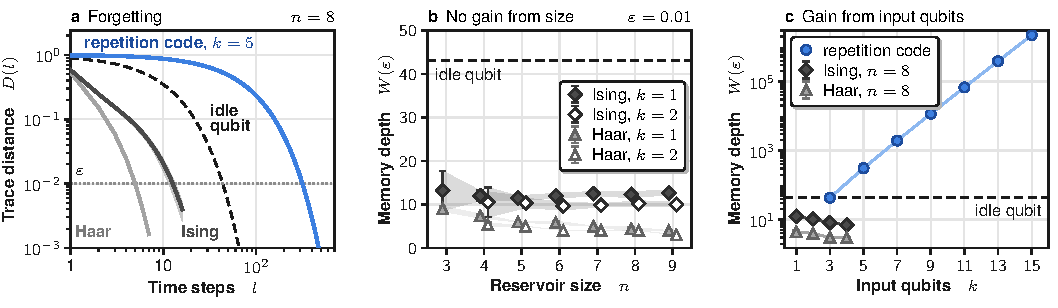
\includegraphics{fig4.pdf}
\caption{\textbf{Standard reservoirs operate far below the memory limit.} Density-matrix simulations at $q=0.9$ with the input encoding of Ref.~\cite{Fujii2017} (Appendix~\ref{app:numerics}).
\pnl{a}~Trace distance $D(l)$ between echo states whose inputs differ only $l+1$ time steps back, for reservoirs with $n=8$ qubits: Haar-random and transverse-field Ising reservoirs with one input qubit (median and range over six realizations), a single qubit that holds the input without repair (idle qubit, dashed), and the repetition-code reservoir with $k=5$ (blue). The memory depth is where $D(l)$ falls below $\varepsilon$ (dotted).
\pnl{b}~Memory depth versus reservoir size for $k=1$ (filled markers) and $k=2$ (open markers); mean and standard deviation over six realizations. The dashed line marks the idle qubit, 43 time steps.
\pnl{c}~Memory depth versus the number of input qubits: Ising and Haar reservoirs with $n=8$, and the repetition-code reservoir with $n=2k-2$ qubits (lower bound from a single-qubit readout).}
\label{fig:numerics}
\end{figure*}

Three observations stand out. First, the memory depth does not grow with the reservoir size [Fig.~\ref{fig:numerics}\,\pnl{b}]. The Ising reservoir remembers about 12 time steps for every $n$ from 3 to 9, and the Haar-random reservoir even forgets faster as it grows, from 9 time steps at $n=3$ to 4 at $n=9$, consistent with noise damping the many-body correlations into which scrambling spreads the input~\cite{Mele2026,Xiong2025}. Second, both stay well below the 43 time steps of a single qubit that simply holds the input. Third, more input qubits shorten their memory [Fig.~\ref{fig:numerics}\,\pnl{c}]. The Ising reservoir with $n=8$ remembers 12 time steps with one input qubit and 7 with four: reinitializing more qubits erases more of the stored information, and neither reservoir uses the fresh qubits to repair what it keeps. The repetition-code reservoir with the same number of qubits, $n=8$, remembers for 316 time steps, and its memory grows exponentially with $k$. Input qubits thus raise the limit, but only dynamics that use them as an entropy sink turn them into memory. In the weak-noise limit, the memory of standard reservoirs saturates at a value set by the reinitialization itself, about 60 time steps on average for the Ising reservoir and 13 for the Haar-random one at $n=6$ (Appendix~\ref{app:numerics}). The gap between standard reservoirs and the limit is a design opportunity rather than a fundamental barrier.

\subsection{Designing reservoirs for time-series forecasting}

Return to the forecasting task~\eqref{eq:task}, and consider two reservoirs with the same noise strength $q=0.9$ and the same $k=2$ input qubits per time step, a reservoir A with $n=20$ qubits and a reservoir B with $n=200$ qubits [Fig.~\ref{fig:overview}\,\pnl{c}]. To forecast $y_{t+1}$, a reservoir must retain $u_{t-100}$, that is, it needs a memory depth of at least 100 time steps at an accuracy that resolves the second term. In fact, it must retain every input of the last 100 time steps at once, a stronger requirement for which the memory depth is necessary but not sufficient. The natural remedy for a reservoir that falls short is to enlarge it. Theorem~\ref{thm:main} shows that this remedy has a limit that does not move with $n$: with two input qubits, the memory depth of every reservoir, A, B, or any larger one, is bounded by the same constant $W_{q,2}(\varepsilon)$, whereas every additional input qubit can multiply the attainable memory depth by a constant factor. Our constants are far too loose to decide whether 100 time steps lie below $W_{0.9,2}(\varepsilon)$; the theorem identifies the knob, not its setting. The simulations add a practical scale: standard Ising reservoirs remember about 12 time steps at this noise level, for every size we could simulate. Four practical lessons follow.

\paragraph*{More qubits are not automatically better.}
A larger reservoir can generate richer features of its recent inputs~\cite{Nakajima2019}, but at fixed $k$ and $q$ its best memory depth is bounded independently of $n$. Large random reservoirs can even suffer from an exponential concentration of their outputs, which makes different inputs hard to distinguish~\cite{Xiong2025,Dao2026}, and they forget faster [Fig.~\ref{fig:numerics}\,\pnl{b}].

\paragraph*{The input-injection architecture is decisive.}
The number of qubits reinitialized per time step sets the limit. More reinitialized qubits do not guarantee a longer memory, however, because reinitialization also erases whatever those qubits stored [Fig.~\ref{fig:numerics}\,\pnl{c}]. The limit is reached only if the reservoir dynamics moves the relevant information out of the input register before it is reinitialized and uses the fresh qubits to repair it, as the repetition-code reservoir does.

\paragraph*{The memory requirement of the task matters.}
If a task depends on inputs further back than the memory depth, no trained readout can recover them. Estimating how far back the task-relevant inputs lie is therefore a prerequisite for choosing $k$.

\paragraph*{A long forecasting horizon is not a long memory.}
Predicting many steps ahead does not by itself require a deep memory; what matters is how far back the inputs lie that determine the target. In Eq.~\eqref{eq:task}, already a one-step forecast requires a memory depth of 100 time steps.

\begin{table*}[t]
\caption{Entropy budget of common ingredients of quantum reservoirs. The budget counts how many bits of purity a process can inject into the reservoir per time step. The memory depth is at most exponential in the total budget, and processes with zero budget cannot extend the memory (Appendix~\ref{app:noise}). Processes outside the model are not covered by the bound.}
\label{tab:budget}
\begin{ruledtabular}
\begin{tabular}{p{5.5cm}p{2.8cm}p{7.9cm}}
{\raggedright Process\par} & {\raggedright Budget per time step\par} & {\raggedright Consequence for the memory\par} \\ \hline
{\raggedright Reinitialization of $k$ input qubits\par} & {\raggedright $k$ bits\par} & {\raggedright memory depth $e^{\Theta(k)}$ under depolarizing noise (Theorem~\ref{thm:main})\par} \\
{\raggedright Measurement followed by reset of $m$ qubits\par} & {\raggedright $m$ bits\par} & {\raggedright counts like $m$ reinitialized input qubits~\cite{Yasuda2023,Hu2024}\par} \\
{\raggedright Unitary input encoding (input-dependent gates)\par} & {\raggedright 0\par} & {\raggedright without another entropy sink, the echo state is the completely mixed state\par} \\
{\raggedright Projective or weak measurement of reservoir qubits whose outcomes only enter the readout\par} & {\raggedright 0\par} & {\raggedright the averaged measurement channel is unital and cannot extend the memory~\cite{Mujal2023}; indirect measurements through fresh meter qubits count like reinitialized qubits~\cite{MorguiSancho2026}\par} \\
{\raggedright Unital noise (Pauli errors, dephasing, coherent errors, crosstalk)\par} & {\raggedright 0\par} & {\raggedright leaves the memory limit unchanged\par} \\
{\raggedright Amplitude damping with probability $\gamma$ on all $n$ qubits\par} & {\raggedright $n\log_2(1+\gamma)$ bits\par} & {\raggedright memory depth can grow exponentially with $n$, already for $k=2$~\cite{BenOr2013,Monzani2024,Freiheit2026}\par} \\
{\raggedright Feedback of measurement outcomes; non-Markovian noise; noise without a depolarizing component\par} & {\raggedright outside the model\par} & {\raggedright memory can be unbounded (Appendix~\ref{app:noise})~\cite{Sannia2026}\par} \\
\end{tabular}
\end{ruledtabular}
\end{table*}

\subsection{An entropy budget for noise and input injection}

The proof of Sec.~\ref{sec:upper} uses only two properties of the noise: a layer of independent depolarizing noise at every time step, and a bound on the purity that a time step can inject. Both survive much additional noise, and the general rule is an entropy budget (Table~\ref{tab:budget}).

\paragraph*{Noise that does not cool the qubits leaves the limit unchanged.}
If the noise at time step $t$ has the form $\mathcal R_t\circ\cD_q^{\otimes n}\circ\mathcal S_t$ with arbitrary unital channels $\mathcal R_t$ and $\mathcal S_t$, Theorem~\ref{thm:main} holds verbatim, even when these channels are correlated across qubits, coherent, input dependent, or drifting in time (Appendix~\ref{app:noise}). This covers Pauli errors, dephasing, coherent over-rotations, and crosstalk. It also covers projective and weak measurements of the reservoir qubits whose outcomes only enter the readout, because the averaged measurement channel is unital; indirect measurements through freshly prepared meter qubits count instead like reinitialized qubits, consistent with the role of measurement back-action as a source of dissipation~\cite{MorguiSancho2026}. Moreover, every unital single-qubit channel with a full-rank Choi matrix, other than complete depolarization, contains a depolarizing component, so independent unital noise on every qubit is always of this form, with an effective noise strength set by the channel.

\paragraph*{Noise that cools the qubits counts as an additional entropy sink.}
A non-unital channel $\mathcal S$ with $\mathcal S(I)\le2^b\,I$ has a budget of $b$ bits: it can inject up to $b$ bits of purity per time step, and the upper bound holds with $k$ replaced by $k+b$. A reset of $m$ qubits after a measurement has $b=m$, so it counts exactly like $m$ reinitialized input qubits. For amplitude damping with probability $\gamma$ on every qubit, $b=n\log_2(1+\gamma)$, so the bound now grows with the reservoir size. This is not an artifact of the proof. Idle qubits relax toward $\ket0$, so a block of qubits left alone for a few time steps becomes a stand-in for freshly reinitialized qubits; this is the quantum-refrigerator mechanism of Ben-Or \emph{et al.}~\cite{BenOr2013}. A reservoir with only two input qubits can use it to reach a memory depth exponential in $n$ (Appendix~\ref{app:noise}). On hardware dominated by energy relaxation, the reservoir size therefore does matter for memory, through cooling. This accounting is consistent with the memory gains attributed to amplitude damping in gate-based reservoirs, where depolarizing and dephasing noise degrade the performance instead~\cite{Monzani2024}, and with collective relaxation as a scalable fading-memory mechanism~\cite{Freiheit2026}. The cooling route is expensive, though. At $q=0.9$ and $\gamma=0.3$, it needs about 1000 qubits to keep the probability of losing the stored bit below $10^{-6}$ per time step with two input qubits, whereas without damping the repetition-code reservoir reaches $1.8\times10^{-7}$ with 32 qubits, 17 of them input qubits~\cite{SM}.

\paragraph*{Where the limit ends.}
Two assumptions cannot be dropped. Under pure dephasing, which has no depolarizing component, computational-basis states never decay, and a reservoir with two input qubits keeps a stored bit forever. And if each qubit suffers a Pauli error that is drawn once and then repeated at every time step, a single time step looks exactly like depolarizing noise on average; yet the errors cancel in pairs, and the reservoir reads the stored bit perfectly at every second time step (Appendix~\ref{app:noise}). Here the environment remembers the noise, which is why the theorem requires Markovian noise. Non-Markovian dynamics can likewise extend the memory of quantum reservoirs in practice~\cite{Sannia2026}. Finally, a reservoir whose measurement outcomes are stored and fed back is coupled to a classical memory outside the model, which is an entropy sink of its own.

\subsection{What the result does not say}

Memory depth is necessary for a temporal task, but it is not sufficient. A reservoir must also transform its input history nonlinearly and make the relevant information visible to its readout~\cite{Cao2026}, and the repetition-code reservoir, whose memory scaling is optimal, computes nothing beyond a delayed copy of its input. Theorem~\ref{thm:main} therefore makes no statement about task performance, nonlinear processing capacity, sampling noise, or a quantum advantage. It bounds how far back any task can reach, not how well a reservoir solves tasks within that range.

In particular, the theorem does not provide an optimal QRC architecture for time series. It does not tell how many input qubits a reservoir of 20 qubits should use, which couplings generate the most useful temporal features~\cite{MartinezPena2021,Cao2026}, how much memory a given real-world time series requires, or when a quantum reservoir outperforms a classical one. The repetition-code reservoir only proves that the exponential scaling can be reached, the constants of the upper bound are conservative by many orders of magnitude, and our simulations cover sizes up to $n=9$. Finally, a long memory does not imply that a reservoir is hard to simulate classically: the reservoir that reaches the limit is described by a single number. The result is thus a fundamental design principle rather than a design recipe.

%======================================================================
\section{Conclusions}
\label{sec:conclusions}
%======================================================================

In this work, we have identified the resource that limits the memory of noisy quantum reservoirs. If $k$ input qubits are reinitialized per time step and every qubit undergoes depolarizing noise, the largest attainable memory depth is $\exp[\Theta(k)]$ time steps, whatever the reservoir dynamics and independent of the total number of qubits. The upper bound follows from a single distance that every noisy time step contracts by a factor depending only on the noise strength and on $k$. A reservoir that stores its input in a repetition code and refreshes it by majority vote reaches the exponential scaling with at most $2k$ qubits. Additional qubits can lengthen the washout of the initial state, but they cannot extend the memory of new inputs. The result extends to an entropy budget: unital noise and measurements of the reservoir qubits without feedback leave the limit unchanged, whereas resets and non-unital noise act as entropy sinks, and energy relaxation can make the memory grow with the reservoir size. Simulations of standard Ising and Haar-random reservoirs show memory depths of a few to about a dozen time steps at $q=0.9$, independent of their size and far below the limit.

For the design of quantum reservoirs, these results make the number of reinitialized qubits per time step, together with the non-unital part of the noise, the parameter that controls memory, and they show that standard reservoir dynamics does not exploit it. When a reservoir forgets too quickly, the first parameter to check is therefore not its size, but its supply of freshly prepared qubits and whether its dynamics uses them. Several questions remain open. The constants of the upper bound are far from tight, and closing the gap between the two exponents would turn the scaling law into a quantitative design rule. Extending the bound to measurement feedback and to non-Markovian noise would cover further experimental platforms. An experiment that varies $k$ at fixed reservoir size could test the predicted scaling directly. Perhaps most relevant for applications is whether natural reservoir dynamics can be engineered to use reinitialized qubits for repair, and whether one can predict, for a given time series, how many reinitialized input qubits a quantum reservoir needs to retain its task-relevant information. Answering these questions would connect the memory limit derived here with concrete reservoir design.

\begin{acknowledgments}
AI-based tools (Claude, Anthropic) assisted with writing and editing the manuscript, checking derivations and references, and implementing the numerical simulations. Markus Baumann checked all results and takes full responsibility for the content of this article.
\end{acknowledgments}

\section*{Data availability}
The code that reproduces all numerical values, simulations, and data figures of this article is provided as Supplemental Material~\cite{SM}.

\appendix

%======================================================================
\section{Norms, purity, and the input budget}
\label{app:norms}
%======================================================================

The proofs use only a few quantities, each with a direct physical meaning. This appendix defines them and collects the elementary facts that the other appendices use.

\subsection{Normalized norms}

For an operator $X$ on $n$ qubits, let $d=2^n$, and let
\begin{equation}
\tau(X)=\frac{\tr(X)}d
\end{equation}
denote the normalized trace, the average of the eigenvalues of $X$; in particular, $\tau(I)=1$. We use the normalized Schatten norms
\begin{equation}
\nrm Xp=\bigl(\tau|X|^p\bigr)^{1/p},\qquad p>0 .
\label{eq:N-norm}
\end{equation}
For $p\ge1$, this is the usual Schatten $p$-norm divided by $d^{1/p}$. The normalization makes $\nrm Ip=1$ for every $p$, so that no factors of $d$ appear in the proofs. For $0<p<1$, we use the same expression, although it is not a norm.

Because $\tau$ averages the eigenvalues of $|X|$, the quantity $\nrm Xp$ is their power mean of order $p$, and it grows with $p$: $\nrm Xp\le\nrm X{p'}$ for $p\le p'$. The 1-norm measures the average size of the eigenvalues, whereas the 2-norm is dominated by the largest ones. Their ratio $\nrm X2/\nrm X1\ge1$ therefore measures how \emph{concentrated} $X$ is. It equals one if all eigenvalues have the same magnitude, and it is large if $X$ is supported on a small subspace. This ratio decides how fast noise erases a difference between two states (Lemma~\ref{lem:forget}).

\subsection{Distinguishability and purity}

Two cases have a direct physical meaning. For the difference of two states, $X=d(\rho-\rho')$, the 1-norm is the trace norm,
\begin{equation}
\nrm X1=\Norm{\rho-\rho'}_1 ,
\end{equation}
twice the trace distance. It measures \emph{distinguishability}: the best measurement tells $\rho$ from $\rho'$ with success probability $\frac12+\frac14\nrm X1$.

For a single state, the 2-norm of $d\rho$ is the purity variable of Sec.~\ref{sec:upper},
\begin{equation}
P=\nrm{d\rho}2=\bigl(d\tr\rho^2\bigr)^{1/2}.
\label{eq:N-purity}
\end{equation}
It equals $1$ for the completely mixed state and $2^{n/2}$ for a pure state. A state with $m$ pure qubits and $n-m$ completely mixed qubits has $P^2=2^m$. In general,
\begin{equation}
\log_2P^2=n-S_2(\rho),
\end{equation}
where $S_2(\rho)=-\log_2\tr\rho^2$ is the R\'enyi-2 entropy in bits. The quantity $\log_2P^2$ thus counts \emph{pure qubits' worth} of purity, however the purity is distributed over the qubits.

\subsection{The input budget}

The input state obeys $0\le\sigma(u)\le I$. The injection step therefore satisfies
\begin{align}
\cE_u(I)&=U\bigl[\sigma(u)\otimes\tr_{\mathrm{in}}I\bigr]U^\dagger\nonumber\\
&=2^k\,U\bigl[\sigma(u)\otimes I\bigr]U^\dagger\le2^k I,
\end{align}
which is Eq.~\eqref{eq:budget}. The factor $2^k$ is the dimension of the discarded input register. Equivalently, $\cE_u(I/d)\le2^kI/d$: starting from the completely mixed state, one time step produces a state whose largest eigenvalue is at most $2^k/d$, that is, whose min-entropy is at least $n-k$ bits. One time step can therefore remove at most $k$ bits of entropy.

The proofs use no other property of the injection step, and the same property describes other processes. We therefore say that a completely positive, trace-preserving (CPTP) map $\cE$ on $n$ qubits has a \emph{budget of $b$ bits} if
\begin{equation}
\cE(I)\le2^b\,I .
\label{eq:A-budgetdef}
\end{equation}
The injection step has a budget of $k$ bits, a unitary or any other unital map has a budget of zero, and a reset of $m$ qubits has a budget of $m$ bits (Appendix~\ref{app:noise}).

\subsection{How a map with a budget acts on the norms}

Every CPTP map $\cE$ with a budget of $b$ bits obeys, for Hermitian $X$,
\begin{equation}
\nrm{\cE X}1\le\nrm X1,\qquad\nrm{\cE X}2\le2^{b/2}\,\nrm X2 .
\label{eq:A-norms}
\end{equation}
The first inequality is the contractivity of the trace norm: no physical process makes two states more distinguishable. For the second, note that $2^{-b}\cE$ is completely positive with $2^{-b}\cE(I)\le I$. The Kadison--Schwarz inequality then gives $(\cE X)^\dagger(\cE X)\le2^b\,\cE(X^\dagger X)$. Applying $\tau$ and using that $\cE$ preserves the trace yields $\nrm{\cE X}2^2\le2^b\nrm X2^2$.

For $X=d\rho$, the second inequality says that a map with a budget of $b$ bits raises $\log_2P^2$ by at most $b$: it adds at most $b$ pure qubits' worth of purity. A unital map, with $b=0$, contracts both norms, which is why unital noise cannot help a reservoir remember (Appendix~\ref{app:noise}).

%======================================================================
\section{Proof of the upper bound}
\label{app:upper}
%======================================================================

This appendix proves the contraction~\eqref{eq:contraction}, from which the upper bound of Theorem~\ref{thm:main} follows (Appendix~\ref{app:washout}). Throughout, $\Nq=\cD_q^{\otimes n}$ denotes one layer of depolarizing noise, and $\cE$ denotes the rest of a time step, a CPTP map with a budget of $b$ bits; for input injection, $b=k$.

The proof has four parts. Two known inequalities about depolarizing noise (Appendices~\ref{app:hyper} and \ref{app:reverse}) give two lemmas: noise caps the purity (Lemma~\ref{lem:cap}), and bounded purity forces forgetting (Lemma~\ref{lem:forget}). Combining the lemmas yields a single distance that every time step contracts (Appendix~\ref{app:contract}). Every constant is derived where it first appears, and Table~\ref{tab:constglossary} collects them all.

\subsection{Hypercontractivity: noise smooths concentrated operators}
\label{app:hyper}

King's hypercontractivity theorem for unital qubit channels~\cite[Corollary~2]{King2014} gives, for every operator $Y$ on $n$ qubits,
\begin{equation}
\nrm{\Nq Y}2\le\nrm Y{1+q^2}.
\label{eq:A-king}
\end{equation}
The theorem bounds $\nrm{\Nq Y}r$ by $\nrm Yp$ whenever $q\le\sqrt{(p-1)/(r-1)}$. Here $r=2$ and $p=1+q^2$, the smallest exponent for which this condition holds.

Because $1+q^2<2$, the norm on the right is weaker than the one on the left. Noise therefore turns operators whose $(1+q^2)$-norm is bounded into operators whose 2-norm is bounded: it smooths out concentrated operators. The mechanism is the damping of correlations. Expand $Y=\sum_Sy_S\,S$ in Pauli strings $S$, and let $|S|$ be the number of qubits on which $S$ acts nontrivially. Noise multiplies each string by $q^{|S|}$. Concentrated operators, such as projectors onto a few states, have expansions that extend to high weights, and these components lose most of their 2-norm.

As a single-qubit check, take $Y=2\ketbra00=I+Z$. Then $\cD_qY=I+qZ$, so $\nrm{\cD_qY}2=(1+q^2)^{1/2}$, whereas $\nrm Y{1+q^2}=2^{q^2/(1+q^2)}$. At $q=0.9$, Eq.~\eqref{eq:A-king} reads $1.345\le1.364$, and it becomes tight in the noiseless limit $q\to1$.

\subsection{Reverse hypercontractivity: noise forces overlap}
\label{app:reverse}

The two-point reverse hypercontractive inequality of Cubitt \emph{et al.}~\cite[Corollary~14]{Cubitt2015} gives, for positive operators $G_1,G_2\ge0$,
\begin{equation}
\tau\bigl[G_1\,\Nq(G_2)\bigr]\ge\nrm{G_1}{\bar p}\,\nrm{G_2}{\bar p},\qquad\bar p=1-q .
\label{eq:A-cubitt}
\end{equation}
The inequality holds for all exponents $\bar p_1,\bar p_2<1$ with $q\le\sqrt{(1-\bar p_1)(1-\bar p_2)}$. We use the symmetric choice $\bar p_1=\bar p_2=1-q$, for which the condition holds with equality.

To read Eq.~\eqref{eq:A-cubitt}, normalize $\tau G=1$, so that $G$ is $d$ times a density matrix. Because $\bar p<1$, the quantity $\nrm G{\bar p}$ then lies between $0$ and $1$. It equals one for $G=I$, and it is small only if $G$ is concentrated on a small subspace. The left-hand side is the overlap of $G_1$ with the noisy version of $G_2$. After one layer of noise, two positive operators therefore overlap substantially unless they are concentrated. Weaker noise means a smaller exponent $\bar p$, which makes $\nrm G{\bar p}$ smaller for concentrated $G$ and the forced overlap weaker.

For two orthogonal single-qubit projectors, $G_1=2\ketbra00$ and $G_2=2\ketbra11$, the left-hand side equals $1-q$ and the right-hand side $2^{-2q/(1-q)}$. Even perfectly distinguishable states overlap after one layer of noise.

\subsection{Lemma 1: noise caps the purity}
\label{app:cap}

\begin{lemma}[Noise caps the purity]\label{lem:cap}
Let $\cE$ have a budget of $b$ bits, and let
\begin{equation}
\theta=\frac{2q^2}{1+q^2},\qquad C=2^{b\theta/2}.
\label{eq:A-thetaC}
\end{equation}
For every Hermitian $X$,
\begin{equation}
\nrm{\Nq\cE X}2\le C\,\nrm X1^{1-\theta}\,\nrm X2^{\theta}.
\end{equation}
\end{lemma}

\paragraph*{Where $\theta$ and $C$ come from.}
Hypercontractivity bounds the 2-norm after the noise by the $(1+q^2)$-norm before it, and the $(1+q^2)$-norm lies between the 1-norm and the 2-norm. H\"older's inequality makes this precise: $\nrm Yp\le\nrm Y1^{1-\theta}\nrm Y2^{\theta}$ whenever $1/p=(1-\theta)+\theta/2$. Setting $p=1+q^2$ and solving for $\theta$ gives Eq.~\eqref{eq:A-thetaC}. The exponent obeys $0<\theta<1$, and $\theta\to1$ as the noise vanishes. The constant $C$ is the factor $2^{b/2}$, by which the step $\cE$ can at most raise the 2-norm, raised to the power $\theta$.

\begin{proof}
By Eq.~\eqref{eq:A-king}, H\"older's inequality, and Eq.~\eqref{eq:A-norms},
\begin{align}
\nrm{\Nq\cE X}2&\le\nrm{\cE X}{1+q^2}\le\nrm{\cE X}1^{1-\theta}\,\nrm{\cE X}2^{\theta}\nonumber\\
&\le\nrm X1^{1-\theta}\bigl(2^{b/2}\nrm X2\bigr)^{\theta}. \qedhere
\end{align}
\end{proof}

\paragraph*{Consequence for the purity.}
For a density matrix, $X=d\rho$ has $\nrm X1=1$, so the purity after one time step obeys $P_t\le C\,P_{t-1}^\theta$, or
\begin{equation}
\log_2P_t\le\theta\log_2P_{t-1}+\frac{b\theta}2 .
\label{eq:A-purityrec}
\end{equation}
For $b=k$, this is Eq.~\eqref{eq:purity}. The log-purity is multiplied by $\theta<1$ at every time step, and the budget adds at most $b\theta/2$. The recursion therefore has the fixed point
\begin{equation}
\log_2P_*=\frac{b\theta}{2(1-\theta)}=\frac{bq^2}{1-q^2},\qquad P_*=C^{1/(1-\theta)},
\label{eq:A-Pstar}
\end{equation}
an upper bound on the purity that a reservoir can maintain. In pure qubits' worth, $\log_2P_*^2=2bq^2/(1-q^2)$, about $8.5$ per bit of budget at $q=0.9$.

\subsection{Lemma 2: bounded purity forces forgetting}
\label{app:forget}

\begin{lemma}[Bounded purity forces forgetting]\label{lem:forget}
Let $Y\ne0$ be traceless and Hermitian, with $y_1=\nrm Y1$ and $y_2=\nrm Y2$, and let
\begin{equation}
a=\frac{2q}{1-q},\qquad c_q=2^{-1/(1-q)} .
\label{eq:A-acq}
\end{equation}
Then
\begin{equation}
\nrm{\Nq Y}1\le y_1\Bigl[1-c_q\Bigl(\frac{y_1}{2y_2}\Bigr)^{a}\Bigr].
\label{eq:A-forget}
\end{equation}
\end{lemma}

In words, one layer of noise removes at least the fraction $c_q(y_1/2y_2)^a$ of the distinguishability. This fraction is small only if the concentration $y_2/y_1$ is large. The proof has three steps, and the constants $a$ and $c_q$ arise in the last one.

\begin{proof}
\emph{(i) Positive and negative parts.} Write $Y=Y_+-Y_-$ with $Y_\pm\ge0$ supported on orthogonal subspaces. Because $Y$ is traceless, $\tau Y_+=\tau Y_-=y_1/2$. The normalized parts $G_\pm=2Y_\pm/y_1$ therefore obey $\tau G_\pm=1$ and $\nrm{G_\pm}2\le2y_2/y_1$.

\emph{(ii) Distinguishability as the error of a test.} A measurement effect $0\le M\le I$ defines a test that guesses ``$+$'' on outcome $M$ and ``$-$'' otherwise. Applied to the noisy parts $\Nq G_\pm$, it errs with total probability
\begin{equation}
\mathrm{err}(M)=\tau\bigl[(I-M)\,\Nq G_+\bigr]+\tau\bigl[M\,\Nq G_-\bigr].
\end{equation}
For Hermitian $Z$, $\tau|Z|=\max_{0\le M\le I}\tau[(2M-I)Z]$. With $Z=\Nq Y=\frac{y_1}2(\Nq G_+-\Nq G_-)$ and $\tau(\Nq G_\pm)=1$, this gives
\begin{equation}
\nrm{\Nq Y}1=y_1\Bigl[1-\min_M\mathrm{err}(M)\Bigr].
\label{eq:A-testerror}
\end{equation}

\emph{(iii) Every test errs.} For every $M$, either $\tau M\ge1/2$ or $\tau(I-M)\ge1/2$. Take the first case; the second is analogous, with $I-M$ and $G_+$ in place of $M$ and $G_-$. Reverse hypercontractivity~\eqref{eq:A-cubitt} gives
\begin{equation}
\mathrm{err}(M)\ge\tau\bigl[M\,\Nq G_-\bigr]\ge\nrm M{\bar p}\,\nrm{G_-}{\bar p},
\end{equation}
and we bound both factors from below.

For the test, $0\le M\le I$ and $\bar p<1$ imply $M^{\bar p}\ge M$, so $\nrm M{\bar p}\ge(\tau M)^{1/\bar p}\ge2^{-1/\bar p}=c_q$. This is the origin of $c_q$: it is the smallest $\bar p$-norm of a test that accepts at least half of the Hilbert space.

For the state part, the function $p\mapsto\ln\tau G^p$ is convex. Writing $1=\lambda\bar p+(1-\lambda)\cdot2$ with $\lambda=1/(2-\bar p)$, convexity gives $1=\tau G\le(\tau G^{\bar p})^{\lambda}(\tau G^2)^{1-\lambda}$ for every $G\ge0$ with $\tau G=1$. Solving for $\nrm G{\bar p}$ yields
\begin{equation}
\nrm G{\bar p}\ge\nrm G2^{-a},\qquad a=\frac{2(1-\bar p)}{\bar p}=\frac{2q}{1-q}.
\end{equation}
This is the origin of $a$: a positive operator whose 2-norm is bounded cannot have a tiny $\bar p$-norm, and $a$ measures how strongly a large 2-norm, that is, concentration, can protect it. With $\nrm{G_-}2\le2y_2/y_1$, we obtain $\nrm{G_-}{\bar p}\ge(y_1/2y_2)^a$.

Altogether, $\mathrm{err}(M)\ge c_q(y_1/2y_2)^a$ for every test, and Eq.~\eqref{eq:A-testerror} proves Eq.~\eqref{eq:A-forget}.
\end{proof}

\subsection{Combining the lemmas: one distance contracts}
\label{app:contract}

Lemma~\ref{lem:forget} needs control of the concentration $y_2/y_1$. Lemma~\ref{lem:cap} provides it, but only for the 2-norm and only up to the factor $C$. We therefore measure the difference $X$ of two states by both norms at once,
\begin{equation}
V(X)=\max\Bigl\{\nrm X1,\ \frac{\nrm X2}{R}\Bigr\},\qquad R=(2C)^{1/(1-\theta)} .
\label{eq:A-V}
\end{equation}
The weight $R$ puts the 2-norm on the scale of the 1-norm. Its value is fixed by a single requirement: one noisy time step must at least halve the 2-norm part of $V$. As shown below, Lemma~\ref{lem:cap} guarantees exactly this for the value of $R$ in Eq.~\eqref{eq:A-V}.

\paragraph*{Contraction.} For every traceless Hermitian $X$,
\begin{equation}
V(\Nq\cE X)\le(1-\delta)\,V(X),\qquad\delta=c_q\bigl(4\cdot2^{b/2}R\bigr)^{-a}.
\label{eq:A-contraction}
\end{equation}
Both sides scale linearly with $X$, so it suffices to consider $V(X)=1$, that is, $\nrm X1\le1$ and $\nrm X2\le R$. We bound the two parts of $V(\Nq\cE X)$ separately.
\begin{itemize}
\item \emph{2-norm part.} Lemma~\ref{lem:cap} gives $\nrm{\Nq\cE X}2/R\le CR^{\theta}/R=C/R^{1-\theta}=1/2$.
\item \emph{1-norm part.} The operator $Y=\cE X$ is traceless, with $y_1\le1$ and, by Eq.~\eqref{eq:A-norms}, $y_2\le2^{b/2}R$. If $y_1\le1/2$, contractivity gives $\nrm{\Nq Y}1\le1/2$. If $y_1>1/2$, then $y_1/2y_2\ge(4\cdot2^{b/2}R)^{-1}$, and Lemma~\ref{lem:forget} gives $\nrm{\Nq Y}1\le1-c_q(4\cdot2^{b/2}R)^{-a}=1-\delta$.
\end{itemize}
Both parts are thus at most $\max\{1/2,1-\delta\}=1-\delta$, because $\delta\le c_q\le1/2$. This proves Eq.~\eqref{eq:A-contraction}, and for $b=k$ the contraction~\eqref{eq:contraction} of the main text. No strong-noise condition is needed, and the argument applies to every map with a budget of $b$ bits, including input-dependent unitaries.

\subsection{The constants of the upper bound}
\label{app:constants}

Inserting $C=2^{b\theta/2}$ into Eq.~\eqref{eq:A-V} gives $R=2^{1/(1-\theta)}P_*$, with $P_*=2^{b\theta/[2(1-\theta)]}$ from Eq.~\eqref{eq:A-Pstar}. The inverse contraction rate is therefore a product of four powers of two,
\begin{equation}
\delta^{-1}=c_q^{-1}\cdot4^a\cdot\bigl(2^{b/2}\bigr)^a\cdot R^a=A_q\,2^{\beta_qb}.
\label{eq:A-deltainv}
\end{equation}
The factors that do not depend on the budget are $c_q^{-1}=2^{1/(1-q)}$, $4^a=2^{2a}$, and the part $2^{a/(1-\theta)}$ of $R^a$. Together they form the prefactor
\begin{equation}
\log_2A_q=\frac1{1-q}+2a+\frac a{1-\theta}=\frac{1}{1-q}\Bigl[1+\frac{2q(3-q^2)}{1-q^2}\Bigr].
\label{eq:A-constants}
\end{equation}
The factors that grow with the budget are $(2^{b/2})^a=2^{ab/2}$ and the part $P_*^a=2^{ab\theta/[2(1-\theta)]}$ of $R^a$. Together they give the exponent
\begin{equation}
\beta_q=\frac a2+\frac{a\theta}{2(1-\theta)}=\frac a{2(1-\theta)}=\frac{q(1+q^2)}{(1-q)(1-q^2)}.
\label{eq:A-beta}
\end{equation}
For $b=k$, this is $\delta^{-1}=A_q2^{\beta_qk}$, the rate in Eqs.~\eqref{eq:upper} and \eqref{eq:contraction}, with the constants of Eq.~\eqref{eq:thmconstants}.

The two constants have a simple meaning. The forgetting time $\delta^{-1}$ grows by the factor $2^{\beta_q}$ for every bit of budget, and $A_q$ collects the factors that do not depend on the budget. Two features of the proof make $\beta_q$ large: Lemma~\ref{lem:forget} is a worst case whose power $a$ grows quickly as the noise weakens, and $V$ lets a single difference use all the purity of the reservoir. At $q=0.9$, $\theta=0.895$, $a=18$, $c_q=2^{-10}$, $\beta_q=85.7$, and $\log_2A_q=217.5$, so $\delta^{-1}=2^{217.5+85.7k}$. Table~\ref{tab:constglossary} lists every constant of the proofs with its origin, and Table~\ref{tab:constants} gives the values for several noise strengths.

\begin{table*}[t]
\caption{Constants of the proofs, where they come from, and their values at $q=0.9$. The budget $b$ is the number of bits of purity that a time step can inject; $b=k$ for input injection.}
\label{tab:constglossary}
\begingroup
\begin{ruledtabular}
\begin{tabular}{p{1.1cm}p{3.3cm}p{9.2cm}p{2.6cm}}
{\raggedright Symbol\par} & {\raggedright Definition\par} & {\raggedright Origin and meaning\par} & {\raggedright $q=0.9$\par} \\ \hline
{\raggedright $\theta$\par} & {\raggedright $2q^2/(1+q^2)$\par} & {\raggedright H\"older exponent in Lemma~\ref{lem:cap}; fraction of the log-purity kept per time step\par} & {\raggedright $0.895$\par} \\
{\raggedright $C$\par} & {\raggedright $2^{b\theta/2}$\par} & {\raggedright prefactor in the interpolated 2-norm bound (Lemma~\ref{lem:cap})\par} & {\raggedright $2^{0.45b}$\par} \\
{\raggedright $P_*$\par} & {\raggedright $2^{bq^2/(1-q^2)}$\par} & {\raggedright fixed point of Eq.~\eqref{eq:A-purityrec}: purity cap of echo states\par} & {\raggedright $2^{4.26b}$\par} \\
{\raggedright $\bar p$\par} & {\raggedright $1-q$\par} & {\raggedright exponent of reverse hypercontractivity\par} & {\raggedright $0.1$\par} \\
{\raggedright $a$\par} & {\raggedright $2q/(1-q)$\par} & {\raggedright power in Lemma~\ref{lem:forget}: protection by concentration\par} & {\raggedright $18$\par} \\
{\raggedright $c_q$\par} & {\raggedright $2^{-1/(1-q)}$\par} & {\raggedright smallest $\bar p$-norm of a test that accepts half of the space\par} & {\raggedright $2^{-10}$\par} \\
{\raggedright $R$\par} & {\raggedright $(2C)^{1/(1-\theta)}$\par} & {\raggedright weight of the 2-norm in $V$; one time step halves $\nrm X2/R$\par} & {\raggedright $2^{9.53+4.26b}$\par} \\
{\raggedright $\delta$\par} & {\raggedright $c_q(4\cdot2^{b/2}R)^{-a}$\par} & {\raggedright fraction of $V$ removed per time step\par} & {\raggedright $2^{-217.5-85.7b}$\par} \\
{\raggedright $\beta_q$\par} & {\raggedright Eq.~\eqref{eq:A-beta}\par} & {\raggedright growth of $\log_2\delta^{-1}$ per bit of budget\par} & {\raggedright $85.7$\par} \\
{\raggedright $A_q$\par} & {\raggedright Eq.~\eqref{eq:A-constants}\par} & {\raggedright budget-independent prefactor of $\delta^{-1}$\par} & {\raggedright $2^{217.5}$\par} \\
{\raggedright $t_0$\par} & {\raggedright $\lceil\ln n/(-\ln\theta)\rceil$\par} & {\raggedright washout time of the purity bound (Appendix~\ref{app:washout})\par} & {\raggedright $42$ for $n=100$\par} \\
{\raggedright $\alpha_q$\par} & {\raggedright $-\frac12\ln(1-q^2)$\par} & {\raggedright decay rate of the majority error (Appendix~\ref{app:lower})\par} & {\raggedright $0.830$\par} \\
{\raggedright $k_q$\par} & {\raggedright $3+\lceil\ln4/\alpha_q\rceil$\par} & {\raggedright sufficient threshold for the lower bound (Appendix~\ref{app:lower})\par} & {\raggedright $5$\par} \\
\end{tabular}
\end{ruledtabular}
\endgroup
\end{table*}

\begin{table}[t]
\caption{Values of the constants for representative noise strengths: the contraction factor $\theta$ of the log-purity; the exponent $\alpha_q$ of the construction, in nats per input qubit; the exponent $\beta_q$ and the prefactor $\log_2A_q$ of the upper bound, in bits; the purity cap $2q^2/(1-q^2)$ of echo states, in pure qubits' worth per input qubit; the washout time $t_0$ of the purity bound for $n=100$; and the threshold $k_q$ of the lower bound.}
\label{tab:constants}
\begin{ruledtabular}
\begin{tabular}{ccccccc}
$q$ & $\theta$ & $\alpha_q$ & $\beta_q$ & $\log_2A_q$ & $\frac{2q^2}{1-q^2}$ & $t_0$, $k_q$ \\ \hline
0.5 & 0.400 & 0.144 & 1.67 & 9.33 & 0.67 & 6, 13 \\
0.8 & 0.780 & 0.511 & 18.2 & 57.4 & 3.56 & 19, 6 \\
0.9 & 0.895 & 0.830 & 85.7 & 217.5 & 8.53 & 42, 5 \\
0.95 & 0.949 & 1.164 & 371 & 837 & 18.5 & 88, 5 \\
0.99 & 0.990 & 1.959 & 9851 & 20198 & 98.5 & 456, 4 \\
\end{tabular}
\end{ruledtabular}
\end{table}

\begin{figure*}[t]
\centering
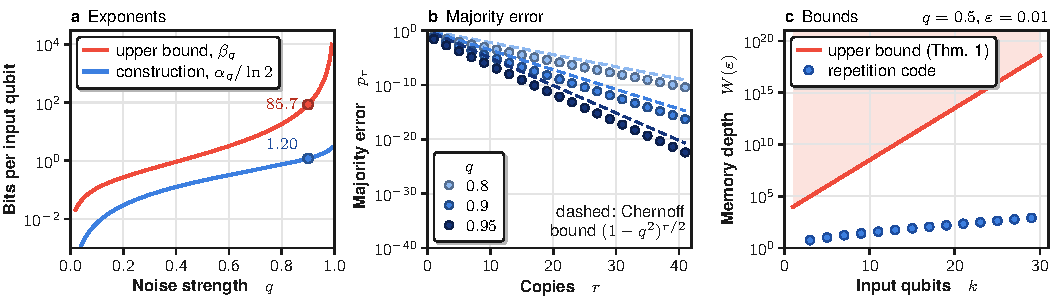
\includegraphics{figA1.pdf}
\caption{\textbf{How tight are the bounds?}
\pnl{a}~Exponents of Theorem~\ref{thm:main} per input qubit: the upper-bound exponent $\beta_q$ and the exponent $\alpha_q/\ln2$ of the repetition-code reservoir, both in bits; dots mark $q=0.9$. The exponent of the construction is the exact asymptotic rate of the majority vote, so the gap between the curves stems from the upper bound.
\pnl{b}~Exact majority error $p_r$ (dots) and the Chernoff bound $(1-q^2)^{r/2}$ (dashed) for three noise strengths. The bound has the exact exponent and overestimates $p_r$ only by a factor polynomial in $r$.
\pnl{c}~Upper bound of Theorem~\ref{thm:main} (line; the shaded region is excluded for every reservoir) and the memory depth of the repetition-code reservoir (dots) at $q=0.5$ and $\varepsilon=0.01$. Both grow exponentially with $k$, at different rates.}
\label{fig:constants}
\end{figure*}

\subsection{How loose is the upper bound?}

Figure~\ref{fig:constants}\,\pnl{a} compares the two exponents. The exponent of the construction is exact for the majority vote [Fig.~\ref{fig:constants}\,\pnl{b}], so the gap stems from the upper bound, mainly from the two features named above. Lemma~\ref{lem:forget} is a worst case over all differences with a given concentration, and its power $a=2q/(1-q)$ grows quickly as the noise weakens. Moreover, $V$ treats the 2-norm as if all of a reservoir's purity could be used to protect a single input.

At $q=0.5$, the upper bound grows by a factor $2^{1.67}$ per input qubit and the construction by a factor $e^{0.144}$; at $q=0.9$, the factors are $2^{85.7}$ and $e^{0.83}$ [Fig.~\ref{fig:constants}\,\pnl{c}]. The scaling with $k$ is nevertheless the same, exponential on both sides, and neither bound depends on $n$.

%======================================================================
\section{Echo states and the washout of the initial state}
\label{app:washout}
%======================================================================

This appendix turns the contraction of Appendix~\ref{app:upper} into the statements about echo states and memory depth used in the main text, and it shows that the washout of the initial state is a separate effect that does grow with $n$.

\subsection{Washout of the purity}

An arbitrary initial state has at most the purity of a pure state, $\log_2P_0\le n/2$. Iterating the purity recursion~\eqref{eq:A-purityrec} gives
\begin{equation}
\log_2P_t\le\theta^t\,\frac n2+(1-\theta^t)\log_2P_*\le\log_2P_*+\theta^t\,\frac n2 .
\label{eq:A-washout}
\end{equation}
The excess purity of the initial state thus decays geometrically, with ratio $\theta$, toward the cap $P_*$. Let
\begin{equation}
t_0=\Bigl\lceil\frac{\ln n}{-\ln\theta}\Bigr\rceil
\end{equation}
be the number of time steps after which $\theta^tn\le1$. For $t\ge t_0$, the initial state contributes at most one pure qubit's worth, $P_t^2\le2P_*^2$. This region is never left again, because one more time step gives at most $C(\sqrt2P_*)^\theta=2^{\theta/2}P_*\le\sqrt2P_*$, where we used $CP_*^\theta=P_*$. At $q=0.9$, $-\ln\theta=0.111$, so $t_0=42$ for $n=100$ and $t_0=63$ for $n=1000$ [Fig.~\ref{fig:contraction}\,\pnl{a}].

\subsection{Unique echo states and the upper bound}

After the washout, any two states are close in the distance $V$. Indeed, if $P_\rho,P_\sigma\le\sqrt2P_*$, then $X=d(\rho-\sigma)$ has $\nrm X1\le2$ and $\nrm X2\le P_\rho+P_\sigma\le2\sqrt2P_*\le2R$, because $R=2^{1/(1-\theta)}P_*\ge2P_*$ (Appendix~\ref{app:constants}). Hence $V(X)\le2$. Let $\Phi_u=\Nq\circ\cE_u$ denote one time step. The contraction~\eqref{eq:A-contraction} then gives, for any two initial states and $L\ge t_0$ time steps,
\begin{equation}
\Norm{\Phi_{u_L}\cdots\Phi_{u_1}(\rho-\sigma)}_1\le2(1-\delta)^{L-t_0}.
\label{eq:A-contract}
\end{equation}
Four consequences follow.
\begin{enumerate}
\item \emph{Echo states exist and are unique.} For a left-infinite input sequence, start the reservoir at progressively earlier times from arbitrary states. By Eq.~\eqref{eq:A-contract}, the resulting states form a Cauchy sequence whose limit does not depend on the initialization. This limit is the unique echo state, and its purity is at most $P_*$.
\item \emph{The upper bound.} Two echo states have purities of at most $P_*$, so their difference has $V\le2$ without any washout. If their input sequences agree on the last $L$ inputs, Eq.~\eqref{eq:A-contract} with $t_0=0$ gives
\begin{equation}
\tfrac12\Norm{\rho(h)-\rho(h')}_1\le(1-\delta)^L\le e^{-\delta L},
\end{equation}
which is Eq.~\eqref{eq:forget}. The memory depth is thus at most $\lceil\delta^{-1}\ln(1/\varepsilon)\rceil$, which is the upper bound~\eqref{eq:upper}.
\item \emph{Finite runs.} A reservoir started in an arbitrary state obeys the same bound at all times $t\ge t_0+W(\varepsilon)$.
\item \emph{No entropy sink, no memory.} For a reservoir with purely unitary input encoding, the budget is zero and $\Phi_u(I/d)=I/d$ for every input. The unique echo state is then $I/d$ for every input sequence.
\end{enumerate}

\begin{figure*}[t]
\centering
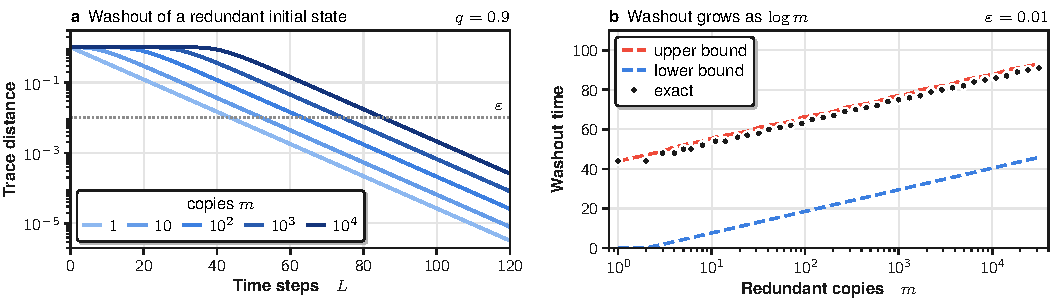
\includegraphics{figA2.pdf}
\caption{\textbf{Two clocks: the washout of the initial state grows with the reservoir size.} A reservoir with $U=I$ whose $m=n-k$ non-input qubits start in $\ket0^{\otimes m}$ or $\ket1^{\otimes m}$, at $q=0.9$.
\pnl{a}~Exact trace distance between the two runs versus time. More copies keep the initial state distinguishable for longer, but every curve eventually decays at the single-qubit rate $q$.
\pnl{b}~Exact washout time to $\varepsilon=0.01$ (dots) together with the upper and lower bounds derived in Appendix~\ref{app:washoutlogn}. All three grow as $\log m$. The memory of new inputs, in contrast, is bounded independently of $n$ (Theorem~\ref{thm:main}).}
\label{fig:washout}
\end{figure*}

\subsection{The washout is necessary, and it grows as \texorpdfstring{$\log n$}{log n}}
\label{app:washoutlogn}

A large reservoir can hold a lot of information about its initial state, which new inputs cannot use. Take $U=I$, and let the $m=n-k$ qubits that are never reinitialized start either in $\ket0^{\otimes m}$ or in $\ket1^{\otimes m}$. After $L$ time steps, every such qubit still shows its initial value with probability $(1+q^L)/2$, independently of the others. The trace distance between the two runs therefore equals the total-variation distance between two binomial distributions, which we evaluate exactly [Fig.~\ref{fig:washout}\,\pnl{a}]. Two simple bounds bracket it.

\paragraph*{Lower bound.} The sum of the $Z$ outcomes has mean $\pm mq^L$ and variance at most $m$. By Chebyshev's inequality, deciding by majority errs with probability at most $1/(mq^{2L})$ under either initialization, so the trace distance is at least $1-2/(mq^{2L})$. It stays above $\varepsilon$ as long as $mq^{2L}>2/(1-\varepsilon)$, that is, for
\begin{equation}
L<\frac{\ln[m(1-\varepsilon)/2]}{2|\ln q|}.
\end{equation}
A washout that grows as $\log m$ is therefore unavoidable.

\paragraph*{Upper bound.} The two product states have fidelity $(1-q^{2L})^{m/2}$, so their trace distance is at most $\sqrt m\,q^L$. It falls below $\varepsilon$ after $\lceil\ln(\sqrt m/\varepsilon)/|\ln q|\rceil$ time steps: copies that are never repaired become indistinguishable after $O_q(\log m)$ time steps.

Both bounds and the exact washout time grow as $\log m$ [Fig.~\ref{fig:washout}\,\pnl{b}]. The same estimate shows that $r$ unrepaired copies of an input keep it readable for only $O_q(\log r)$ time steps, as stated in Sec.~\ref{sec:lower}.

%======================================================================
\section{The repetition-code reservoir}
\label{app:lower}
%======================================================================

This appendix derives the exact response of the reservoir of Sec.~\ref{sec:lower} and the lower bound of Theorem~\ref{thm:main}, including the origin of the constants $\alpha_q$ and $k_q$.

\subsection{The construction}

The reservoir has $n=2r+2$ qubits: an input register of $k=r+2$ qubits, consisting of the two input qubits $(c,b)$ and $r$ ancillas, and $r$ memory qubits. The unitary~\eqref{eq:repU} permutes computational basis states. It is invertible, because its output reveals $x$, $c$, and $b$, hence $F_{c,b}(x)$, and hence $z$. A permutation of basis states is a unitary. A blank input injects $\ket{0,0}$ into $(c,b)$ and $\ket0^{\otimes r}$ into the ancillas; a bit $b$ to be stored injects $\ket{1,b}$ and $\ket0^{\otimes r}$.

\subsection{Exact response}

Under depolarizing noise, a qubit in $\ket0$ or $\ket1$ flips with probability $p=(1-q)/2$ and is otherwise left alone. Diagonal states thus stay diagonal, and every qubit behaves as a classical bit. Let $\hat b_j$ denote the bit that the unitary writes into the ancillas at time step $j$. During a blank time step, $\hat b_j=\mathrm{maj}(x)$, where $x$ are the copies written at time step $j-1$, each of which has flipped with probability $p$ during one round of noise, independently of the others. Hence $\Pr[\hat b_j\ne\hat b_{j-1}]=p_r$ for either value of $\hat b_{j-1}$, and
\begin{equation}
\mathbb E\bigl[(-1)^{\hat b_j}\bigr]=\lambda_r\,\mathbb E\bigl[(-1)^{\hat b_{j-1}}\bigr],\qquad\lambda_r=1-2p_r .
\end{equation}
A stored bit sets $\hat b=b$ exactly, after which the bias decays as $\lambda_r^{\,t}$. Each memory qubit equals the current bit $\hat b$ up to one round of noise, which contributes the factor $q$ in Eq.~\eqref{eq:response}.

\subsection{The majority error and the exponent \texorpdfstring{$\alpha_q$}{alpha q}}

The majority of $r$ copies, for odd $r$, is wrong if more than half of them have flipped. Write $\xi_i=+1$ if copy $i$ is intact and $\xi_i=-1$ if it has flipped, so that the $\xi_i$ are independent with mean $q$. For every $\eta>0$, Markov's inequality applied to $e^{-\eta\sum_i\xi_i}$ gives the Chernoff bound
\begin{equation}
p_r=\Pr\Bigl[\sum_i\xi_i<0\Bigr]\le\Bigl[\tfrac{1+q}2e^{-\eta}+\tfrac{1-q}2e^{\eta}\Bigr]^r.
\end{equation}
The choice $e^{2\eta}=(1+q)/(1-q)$ minimizes the bracket, which then equals $\sqrt{1-q^2}$. Hence
\begin{equation}
p_r\le(1-q^2)^{r/2}=e^{-\alpha_qr},\qquad\alpha_q=-\tfrac12\ln(1-q^2),
\label{eq:A-chernoff}
\end{equation}
which is Eq.~\eqref{eq:pr}. This is the origin of $\alpha_q$: it is the rate at which the majority vote becomes reliable as copies are added. The rate is exact, since $p_{r+2}/p_r\to1-q^2$ for large $r$; the Chernoff bound overestimates $p_r$ only by a factor polynomial in $r$ [Fig.~\ref{fig:constants}\,\pnl{b}].

By Bernoulli's inequality, $\lambda_r^{\,t}\ge1-2tp_r\ge1/2$ for $t\le e^{\alpha_qr}/4$, so the half-life of a stored bit is at least $e^{\alpha_qr}/4$. Table~\ref{tab:halflife} lists exact half-lives for several noise strengths.

\begin{table}[b]
\caption{Exact half-lives (in time steps) of a bit stored in the repetition-code reservoir, the largest $T$ with $\lambda_r^T\ge1/2$, for $k=r+2$ input qubits and several noise strengths~\cite{SM}.}
\label{tab:halflife}
\begin{ruledtabular}
\begin{tabular}{cccccc}
$q$ & $k=3$ & $k=5$ & $k=9$ & $k=13$ & $k=17$ \\ \hline
0.8 & 3 & 12 & 126 & 1171 & 10\,306 \\
0.9 & 6 & 47 & 1790 & 59\,739 & $1.9\times10^{6}$ \\
0.95 & 13 & 187 & 26\,931 & $3.4\times10^{6}$ & $4.1\times10^{8}$ \\
0.99 & 68 & 4636 & $1.6\times10^{7}$ & $4.9\times10^{10}$ & $1.4\times10^{14}$ \\
\end{tabular}
\end{ruledtabular}
\end{table}

\subsection{The lower bound and the threshold \texorpdfstring{$k_q$}{k q}}
\label{app:lowerbound}

Two input sequences that differ only in the bit stored $L$ time steps ago, followed by blanks, agree on their last $L$ inputs. By Eq.~\eqref{eq:response}, their echo states give expectation values of $Z$ on a memory qubit that differ by $2q\lambda_r^L$. Since $|\tr[O(\rho-\rho')]|\le\Norm O\,\Norm{\rho-\rho'}_1$, their trace distance is at least $q\lambda_r^L$, which exceeds $\varepsilon$ as long as $L<\ln(q/\varepsilon)/(-\ln\lambda_r)$. This gives the first inequality in Eq.~\eqref{eq:lower}; it requires $\varepsilon<q$, because the readout qubit's own last round of noise contributes the factor $q$.

For the second inequality, we use $-\ln(1-x)\le2x$ for $0\le x\le1/2$, with $x=2p_r$. This requires $p_r\le1/4$, and then $-\ln\lambda_r\le4p_r\le4e^{-\alpha_qr}$ by Eq.~\eqref{eq:A-chernoff}.

For a general number $k$ of input qubits, we choose $r$ as the largest odd number with $r\le k-2$ and leave the remaining input qubits unused. Then $r\ge k-3$ and $n=k+r\le2k$, so Eq.~\eqref{eq:lower} gives Eq.~\eqref{eq:lowerthm}. The condition $p_r\le1/4$ holds if $e^{-\alpha_qr}\le1/4$, that is, if $r\ge\ln4/\alpha_q$. Since $r\ge k-3$, it is guaranteed for
\begin{equation}
k\ge k_q=3+\Bigl\lceil\frac{\ln4}{\alpha_q}\Bigr\rceil .
\end{equation}
The threshold $k_q$ is thus a sufficient number of input qubits for the majority vote to be reliable enough for this estimate; at $q=0.9$, $k_q=5$. Finally, a stored bit overwrites the memory qubits regardless of their previous state. The two input sequences therefore lead to valid echo states, and the memory is not a remnant of the initialization.

\subsection{The single-qubit readout is nearly optimal}

The lower bound uses the readout of a single memory qubit. The full reservoir state carries slightly more information: for $k=5$ and $q=0.9$, the trace distance between the two echo states [Fig.~\ref{fig:numerics}\,\pnl{a}] gives a memory depth of 316 time steps at $\varepsilon=0.01$, compared with 308 from Eq.~\eqref{eq:lower}.

\subsection{Retention cost}

Suppose a reservoir must keep the readouts for a stored 0 and a stored 1 at least $q$ apart for $T$ time steps. Equation~\eqref{eq:forget} bounds this gap by $2e^{-\delta T}$, so $T\le\delta^{-1}\ln(2/q)$ and, with $\delta^{-1}=A_q2^{\beta_qk}$, $k=\Omega_q(\log T)$. Conversely, Eq.~\eqref{eq:response} keeps the gap for all $t\le T$ if $T\le e^{\alpha_qr}/4$. An odd $r\ge\ln(4T)/\alpha_q$ and $k=r+2$ therefore suffice, so $k=O_q(\log T)$.

\subsection{Anisotropic noise}

For independent unital noise $\mathcal M$ on every qubit, the bit is best stored along the Bloch axis that $\mathcal M$ preserves best. Let $s_{\mathcal M}$ be the largest singular value of the matrix by which $\mathcal M$ acts on Bloch vectors, with unit vectors $\bm v$ and $\bm v'$ such that $\mathcal M$ maps the Bloch vector $\bm v$ to $s_{\mathcal M}\bm v'$. Conjugating the memory block of Eq.~\eqref{eq:repU} by single-qubit rotations from the $\bm v'$ basis and into the $\bm v$ basis makes every memory qubit an independent copy of the stored bit, flipped with probability $(1-s_{\mathcal M})/2$. The lower bound then holds with $q$ replaced by $s_{\mathcal M}$.

%======================================================================
\section{Entropy budget beyond depolarizing noise}
\label{app:noise}
%======================================================================

This appendix extends Theorem~\ref{thm:main} to more general noise, using the budget of Appendix~\ref{app:norms}, and shows where the extension ends.

\subsection{Unital noise and measurements}

Let the noise at time step $t$ be $\mathcal R_t\circ\Nq\circ\mathcal S_t$, where $\mathcal R_t$ and $\mathcal S_t$ are unital channels. They may be correlated across qubits, coherent, input dependent, or drifting in time. Two observations reduce this case to the one already proven.
\begin{enumerate}
\item The channel $\mathcal S_t$ can be absorbed into the injection step. The map $\mathcal S_t\circ\cE_u$ is CPTP, and because $\mathcal S_t$ is positive and unital, $\mathcal S_t\cE_u(I)\le2^k\mathcal S_t(I)=2^kI$. It therefore has the same budget, $k$ bits.
\item The channel $\mathcal R_t$ cannot increase $V$, because a unital map contracts both norms [Eq.~\eqref{eq:A-norms} with $b=0$].
\end{enumerate}
Hence $V(\mathcal R_t\Nq\mathcal S_t\cE_uX)\le V(\Nq\mathcal S_t\cE_uX)\le(1-\delta)V(X)$, and the same two facts give the purity recursion. Two input sequences that agree on their last $L$ inputs share every map during those $L$ time steps, so Theorem~\ref{thm:main} holds verbatim. Its lower bound needs only $\mathcal R_t=\mathcal S_t=\mathrm{id}$.

Measurements are covered in the same way. An unconditional measurement with Kraus operators $\sqrt{E_i}$, projective or weak, is unital, because $\sum_i\sqrt{E_i}\sqrt{E_i}=\sum_iE_i=I$. Measurements of the reservoir qubits whose outcomes only enter the readout therefore cannot extend the memory. An indirect measurement through a meter qubit that is freshly prepared at every time step is different: the meter is a reinitialized qubit and adds one bit of budget per time step.

\subsection{Non-unital noise and resets}

Now let $\mathcal R_t$ and $\mathcal S_t$ be arbitrary channels with budgets of $b_R$ and $b_S$ bits, $\mathcal R_t(I)\le2^{b_R}I$ and $\mathcal S_t(I)\le2^{b_S}I$, with $\mathcal R_t$ independent of the inputs. Regroup the time steps as $\rho_t=\mathcal R_t(\tilde\rho_t)$, with
\begin{equation}
\tilde\rho_t=\Psi_t(\tilde\rho_{t-1}),\qquad\Psi_t=\Nq\circ\mathcal S_t\circ\cE_{u_t}\circ\mathcal R_{t-1},
\end{equation}
and $\mathcal R_0=\mathrm{id}$. By positivity, $\mathcal S_t\cE_{u_t}\mathcal R_{t-1}(I)\le2^{k+b_R+b_S}I$, so Appendices~\ref{app:upper} and \ref{app:washout} apply to $\tilde\rho_t$ with the budget $b=k+b_R+b_S$. Two input sequences that agree on their last $L$ inputs share every $\Psi_t$ during those $L$ time steps. The final channel $\mathcal R_t$ cannot increase trace distances, so the memory depth of $\rho_t$ is at most that of $\tilde\rho_t$. Apart from the washout time, the reservoir size thus enters only through $b_R+b_S$. The bounds hold for every realization of random noise, and hence also on average.

The main text uses two budgets. A reset channel $\rho\mapsto\tr(\rho)\ketbra00$ maps $I$ to $2\ketbra00\le2I$, so a reset of $m$ qubits has a budget of $m$ bits. Amplitude damping $\AD_\gamma$ with probability $\gamma$ maps $I$ to $\mathrm{diag}(1+\gamma,1-\gamma)\le(1+\gamma)I$, so a layer of amplitude damping on all $n$ qubits has a budget of $n\log_2(1+\gamma)$ bits.

\subsection{Unital qubit channels with full-rank Choi matrices contain depolarizing noise}

Let $\mathcal M$ be a unital qubit channel, and let
\begin{equation}
\Omega_{\mathcal M}=\sum_{i,j=0}^1\mathcal M\bigl(\ketbra ij\bigr)\otimes\ketbra ij
\end{equation}
be its Choi matrix, a positive operator with $\tr\Omega_{\mathcal M}=2$. Complete depolarization, $\cD_0(X)=\tr(X)I/2$, has $\Omega_{\cD_0}=I/2$. Suppose that $\Omega_{\mathcal M}$ is positive definite and that $\mathcal M\ne\cD_0$. Then the smallest eigenvalue of $\Omega_{\mathcal M}$ lies in $(0,1/2)$, and
\begin{equation}
q_{\mathcal M}=1-2\lambda_{\min}(\Omega_{\mathcal M})\in(0,1).
\end{equation}
The map $\mathcal T=[\mathcal M-(1-q_{\mathcal M})\cD_0]/q_{\mathcal M}$ is trace preserving and unital, and its Choi matrix $[\Omega_{\mathcal M}-\lambda_{\min}(\Omega_{\mathcal M})I]/q_{\mathcal M}$ is positive semidefinite, so $\mathcal T$ is a channel. Because $\mathcal T\circ\cD_q=q\mathcal T+(1-q)\cD_0$ for every unital channel $\mathcal T$, we obtain
\begin{equation}
\mathcal M=\mathcal T\circ\cD_{q_{\mathcal M}} .
\end{equation}
Every such channel is thus depolarizing noise of strength $q_{\mathcal M}$ followed by a unital channel, which is the form covered above. For a Pauli channel with probabilities $p_I,p_X,p_Y,p_Z$, the Choi eigenvalues are $2p_I,\dots,2p_Z$, so $1-q_{\mathcal M}=4\min\{p_I,p_X,p_Y,p_Z\}$. For example, Pauli noise with $p_X=p_Y=0.01$ and $p_Z=0.08$ has $q_{\mathcal M}=0.96$.

\begin{figure*}[t]
\centering
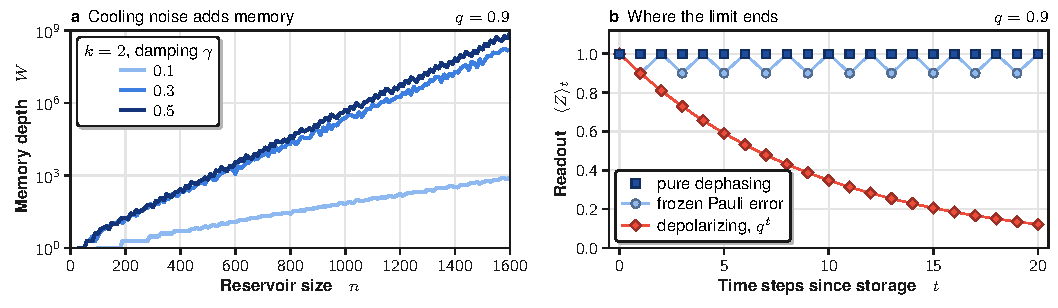
\includegraphics{figA3.pdf}
\caption{\textbf{The entropy budget at work.}
\pnl{a}~Cooling noise adds memory. Lower bound $\lfloor1/(4p_{\mathrm f})\rfloor$ on the memory depth of the cooling reservoir of Appendix~\ref{app:cooling}, with only $k=2$ input qubits, under the noise $(\cD_q\circ\AD_\gamma)^{\otimes n}$ at $q=0.9$. Here $p_{\mathrm f}$ is the worst-case probability of losing the stored bit per time step, computed from exact binomial tails and optimized over the cooling time $s$. The memory grows exponentially with $n$ because amplitude damping supplies $n\log_2(1+\gamma)$ bits of purity per time step.
\pnl{b}~Where the limit ends. Readout of a stored bit under pure dephasing (no decay), under a Pauli error that is drawn once and then repeated at every time step (perfect revivals at every second time step, although one time step is depolarizing on average), and under Markovian depolarizing noise ($q^t$).}
\label{fig:budget}
\end{figure*}

\subsection{Cooling noise: memory exponential in \texorpdfstring{$n$}{n}}
\label{app:cooling}

Amplitude damping can make the memory grow with the reservoir size, already with two input qubits. The construction uses idle qubits as a refrigerator~\cite{BenOr2013}. Let every time step end with the noise $(\cD_q\circ\AD_\gamma)^{\otimes n}$.

\paragraph*{Idle qubits cool.}
On diagonal states, one time step of noise acts on every qubit as a bit channel: a qubit that is 1 with probability $x$ becomes 1 with probability
\begin{equation}
p+\kappa x,\qquad p=\frac{1-q}2,\qquad\kappa=q(1-\gamma).
\end{equation}
Here $p$ is the flip probability of depolarizing noise, as in Sec.~\ref{sec:lower}, and $\kappa<1$ is the fraction of a qubit's polarization that survives one time step. A qubit left alone approaches the stationary probability $p_\infty=p/(1-\kappa)$ of being 1, which is below $1/2$ for every $\gamma>0$: idle qubits cool. After $s$ time steps, starting from either value, a qubit is 1 with probability at most
\begin{equation}
\mu_s=p_\infty+\kappa^s(1-p_\infty),
\end{equation}
and we choose the cooling time $s$ such that $\mu_s<1/2$.

\paragraph*{The reservoir.}
The reservoir has the two input qubits $(c,b)$ of Sec.~\ref{sec:lower} and $s+1$ blocks $x_0,\dots,x_s$ of $r=\lfloor(n-2)/(s+1)\rfloor$ qubits each. Block $x_0$ holds the stored bit, and the other blocks form a queue in which qubits cool. The reservoir unitary is the basis permutation
\begin{align}
U\ket{c,b}&\ket{x_0,x_1,\dots,x_s}\nonumber\\
&=\ket{c,b}\ket{x_s\oplus F_{c,b}(x_0)\bm1,\,x_0,\dots,x_{s-1}}.
\end{align}
For a store input, $F_{1,b}(x)=b$. For a blank input, $F_{0,b}(x)=1$ if the fraction of ones in $x$ is at least the threshold $\chi=p+\kappa/2$, and $F_{0,b}(x)=0$ otherwise. In words, $U$ decodes the stored bit by a threshold vote, writes it into the coolest block $x_s$, and moves the other blocks one position along the queue.

\paragraph*{Error per time step.}
The reused block has cooled for $s$ time steps, so each of its bits differs from the newly written bit $F$ with probability at most $\mu_s$, independently given the past. After the noise, each bit of the new memory block is therefore 1 with probability at least $p+\kappa(1-\mu_s)$ if $F=1$, and at most $p+\kappa\mu_s$ if $F=0$. The threshold $\chi$ lies between these two values, at a distance of at least $\kappa(1/2-\mu_s)$ from both. The next vote therefore errs with probability at most
\begin{align}
p_{\mathrm f}=\max\bigl\{&\Pr[\mathrm{Bin}(r,p+\kappa\mu_s)\ge\chi r],\nonumber\\
&\Pr[\mathrm{Bin}(r,p+\kappa(1-\mu_s))<\chi r]\bigr\},
\end{align}
and Hoeffding's inequality~\cite{Hoeffding1963} gives $p_{\mathrm f}\le e^{-\nu r}$ with $\nu=2\kappa^2(1/2-\mu_s)^2$. The failure probability thus falls exponentially with the block size.

\paragraph*{Memory.}
Consider two input sequences that differ only in the bit stored $L$ time steps ago, followed by blanks. The stored bit survives the $L+1$ subsequent votes with probability at least $1-(L+1)p_{\mathrm f}$, so the threshold observable of block $x_0$ ($+1$ if the fraction of ones is at least $\chi$, $-1$ otherwise) differs between the two echo states by at least $2-4(L+1)p_{\mathrm f}$. For $(L+1)p_{\mathrm f}\le1/4$, this difference is at least $1$, and the trace distance is at least $1/2$. Hence
\begin{equation}
W(\varepsilon)\ge\Bigl\lfloor\frac1{4p_{\mathrm f}}\Bigr\rfloor\ge\Bigl\lfloor\frac{e^{\nu r}}4\Bigr\rfloor\qquad\text{for all }\varepsilon<\frac12 .
\end{equation}
With only two input qubits, the memory depth is exponential in $r\approx n/(s+1)$, and hence in $n$ [Fig.~\ref{fig:budget}\,\pnl{a}].

\paragraph*{Numbers.}
At $q=0.9$ and $\gamma=0.3$, we have $p=0.05$, $\kappa=0.63$, and $p_\infty\approx0.135$. The exact binomial tails, optimized over the cooling time $s$, push $p_{\mathrm f}$ below $10^{-6}$ at $n=1010$ qubits, with $s=7$ and $r=126$.

\subsection{Two counterexamples}

Two assumptions of Theorem~\ref{thm:main} cannot be dropped: that the noise has a depolarizing component, and that it is Markovian. Consider a single memory qubit next to the two input qubits $(c,b)$. The reservoir unitary swaps $b$ into the memory qubit when $c=1$ and acts trivially when $c=0$; the old memory value leaves with the input register at the next input injection.

\paragraph*{Pure dephasing.}
Under the dephasing channel $\mathcal Z_\phi(X)=(1-\phi)X+\phi\,ZXZ$, computational-basis states are fixed points, so a stored bit stays perfectly readable forever.

\paragraph*{Frozen Pauli errors.}
Let each qubit carry a Pauli operator $S\in\{I,X,Y,Z\}$, drawn once with probabilities $\frac{1+3q}4,\frac{1-q}4,\frac{1-q}4,\frac{1-q}4$ and then applied at every time step. Averaged over the draw, one time step is exactly $\cD_q^{\otimes n}$, because
\begin{equation}
\mathbb E[S\rho S]=\tfrac{1+3q}4\rho+\tfrac{1-q}4(X\rho X+Y\rho Y+Z\rho Z)=\cD_q(\rho).
\end{equation}
But $S^2=I$, so after an even number of time steps the memory qubit is back in $\ketbra bb$, and the stored bit is read perfectly at every second time step. Averaged over the draw, the readout alternates between $1$ and $q$ [Fig.~\ref{fig:budget}\,\pnl{b}]. Here the environment remembers the noise.

In both cases, the reservoir has no unique echo state, and no finite memory depth exists for input sequences that contain a stored bit.

%======================================================================
\section{Numerical simulations}
\label{app:numerics}
%======================================================================

\begin{figure*}[t]
\centering
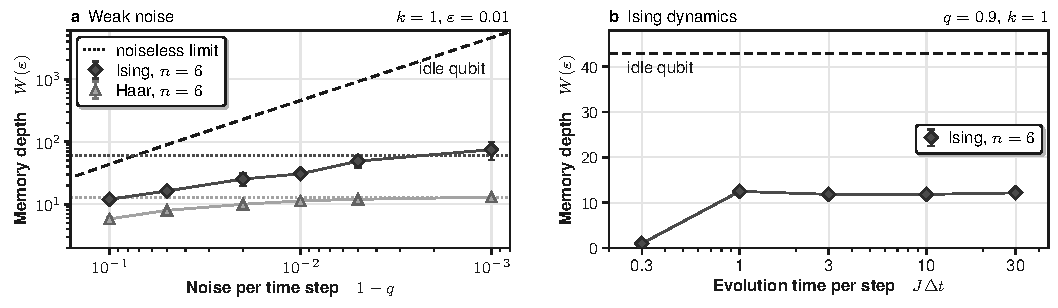
\includegraphics{figA4.pdf}
\caption{\textbf{The memory of standard reservoirs is robust and saturates without noise.}
\pnl{a}~Memory depth of Ising and Haar reservoirs with $n=6$ and $k=1$ versus the noise per time step (mean and standard deviation over realizations), compared with an idle qubit (dashed). Dotted lines: the noiseless limit $q=1$, in which the reinitialization of the input qubit is the only source of forgetting.
\pnl{b}~Memory depth of the Ising reservoir versus the evolution time per time step at $q=0.9$. For $J\Delta t\gtrsim1$ the memory depth is about 12 time steps; for short evolution times, the input never leaves the input register and is erased at the next injection.}
\label{fig:robust}
\end{figure*}

\subsection{Reservoirs}

We simulate the density matrix of Eq.~\eqref{eq:model} exactly for $n\le9$ qubits. The first $k$ qubits form the input register. Each input qubit is reinitialized in $\ket{\psi(u_t)}=\sqrt{1-u_t}\,\ket0+\sqrt{u_t}\,\ket1$~\cite{Fujii2017}, with independent inputs $u_t$ drawn uniformly from $[0,1]$. We consider two reservoir unitaries.
\begin{itemize}
\item The \emph{Ising reservoir} evolves for a time $\Delta t$ under the transverse-field Ising Hamiltonian
\begin{equation}
H=\sum_{i<j}J_{ij}X_iX_j+g\sum_iZ_i,
\end{equation}
with couplings $J_{ij}$ drawn uniformly from $[-J/2,J/2]$, transverse field $g=J$, and $J\Delta t=10$, as in the standard model of QRC~\cite{Fujii2017,Nakajima2019,MartinezPena2021}.
\item The \emph{Haar reservoir} uses a unitary drawn from the Haar measure on $U(2^n)$, the extreme of information scrambling.
\end{itemize}
After every time step, each qubit undergoes depolarizing noise $\cD_q$. Table~\ref{tab:sim} lists all parameters.

\begin{table}[!tb]
\caption{Parameters of the simulations in Fig.~\ref{fig:numerics} and Fig.~\ref{fig:robust}.}
\label{tab:sim}
\begin{ruledtabular}
\begin{tabular}{p{3.2cm}p{4.4cm}}
{\raggedright Parameter\par} & {\raggedright Value\par} \\ \hline
{\raggedright Noise strength $q$\par} & {\raggedright $0.9$; also $0.95$--$1$ (Fig.~\ref{fig:robust})\par} \\
{\raggedright Accuracy $\varepsilon$\par} & {\raggedright $0.01$\par} \\
{\raggedright Reservoir size $n$\par} & {\raggedright 3--9\par} \\
{\raggedright Input qubits $k$\par} & {\raggedright 1--4\par} \\
{\raggedright Ising couplings\par} & {\raggedright $J_{ij}\in[-J/2,J/2]$, field $g=J$\par} \\
{\raggedright Evolution time\par} & {\raggedright $J\Delta t=10$; also 0.3--30 (Fig.~\ref{fig:robust})\par} \\
{\raggedright Input encoding\par} & {\raggedright $\sqrt{1-u}\,\ket0+\sqrt u\,\ket1$, $u\in[0,1]$\par} \\
{\raggedright Washout\par} & {\raggedright 60--80 time steps\par} \\
{\raggedright Continuations\par} & {\raggedright 5 per realization\par} \\
{\raggedright Realizations\par} & {\raggedright 6 (3 for $q>0.9$)\par} \\
{\raggedright Stopping criterion\par} & {\raggedright $D(l)<3\times10^{-3}$\par} \\
\end{tabular}
\end{ruledtabular}
\end{table}

\subsection{Memory depth}

Because each time step is linear, the difference $\Delta_l$ of two reservoir states evolves under the same map as the states themselves. For each realization, we run the reservoir from the completely mixed state for a washout period with random inputs. We then inject the two most different inputs, $u=0$ and $u=1$, into two copies of the same state. Their difference evolves under a common continuation of the input sequence, and we record $D(l)=\frac12\Norm{\Delta_l}_1$ after $l$ further time steps, until $D(l)$ falls below $3\times10^{-3}$, well below $\varepsilon$.

We use five continuations per realization: two random input sequences and the constant inputs $u=0$, $1/2$, and $1$. The memory depth of a realization is $1+\max\{l:D(l)>\varepsilon\}$, maximized over the continuations. Since the memory depth is a supremum over all input histories, this estimate is a lower bound on the true memory depth of each reservoir.

\subsection{Validation}

Three checks confirm the code.
\begin{enumerate}
\item The evolution of differences agrees with the difference of evolved states to machine precision.
\item For the repetition-code reservoir, the simulated single-qubit readout reproduces the exact response $q\lambda_r^l$ of Eq.~\eqref{eq:response} to machine precision for $r=1$ and $r=3$.
\item After the washout of 60 time steps, runs from the completely mixed state and from two different pure product states agree within a trace distance of $10^{-6}$, far below $\varepsilon$.
\end{enumerate}

\subsection{Robustness}

The conclusions of Sec.~\ref{sec:numerics} do not depend on the parameters (Fig.~\ref{fig:robust}). As the noise weakens, the memory depth of standard reservoirs grows far more slowly than that of an idle qubit, which grows as $1/(1-q)$, and it saturates in the noiseless limit [Fig.~\ref{fig:robust}\,\pnl{a}]. There, the reinitialization of the input register is the only source of forgetting: every time step discards the part of the stored information that the dynamics has moved into the input register. Even a noiseless reservoir therefore forgets, within 40 to 95 time steps for our Ising realizations and within 13 time steps for the Haar-random ones at $n=6$.

For the Ising reservoir, the memory depth is insensitive to the evolution time once $J\Delta t\gtrsim1$ [Fig.~\ref{fig:robust}\,\pnl{b}]. For very short evolution times, the input never leaves the input register, so the reservoir forgets it at the next injection.


\bibliography{refs}

\end{document}
